%\documentclass[first,firstsupp,handout,compress,notes,navigation]{ETHclass} 
%\documentclass[first,firstsupp,handout,lastsupp]{ETHclass} 
\documentclass[first,firstsupp,lastsupp,handout,last,hyperref,table]{ETHclass} 
%\documentclass[first,firstsupp]{ETHclass}
\usepackage{etex}

\usepackage{adjustbox}
\usepackage{amsmath}
\usepackage{amssymb}
\usepackage{animate}
\usepackage{booktabs}
\usepackage{charter}
\usepackage{enumitem}
\usepackage{etoolbox}
\usepackage{ifthen}
\usepackage{longtable}
\usepackage{mathrsfs}
\usepackage{multicol}
\usepackage{pgf}
\usepackage{pgfplots}
\usepackage{pifont}
\usepackage{ragged2e}
\usepackage{standalone}
\usepackage[caption=false]{subfig}
\usepackage{tabularx}
\usepackage{tikz}
\usepackage{verbatim}
\usepackage{xcolor}
\usepackage{hyperref}

\pgfplotsset{compat=1.7}

\setbeamertemplate{navigation symbols}{}
\usetikzlibrary{arrows,decorations.pathreplacing,positioning,shapes,shadows}

%\usepackage[style=numeric-comp]{biblatex}

%\usepackage{lipsum}

%\usetikzlibrary{fit}
\usetikzlibrary{arrows}
\usetikzlibrary{trees}

% Options for beamer:
%
% 9,10,11,12,13,14,17pt  Fontsizes
% 
% compress: navigation bar becomes smaller
% t       : place contents of frames on top (alternative: b,c)
% handout : handoutversion
% notes   : show notes
% notes=onlyslideswithnotes
%
%hyperref={bookmarksopen,bookmarksnumbered} : Needed for menues in
%                                             acrobat. Also need
%                                             pdftex as option or 
%                                             compile with
% pdflatex '\PassOptionsToPackage{pdftex,bookmarksopen,bookmarksnumbered}{hyperref} \input{file}'

%\usepackage{beamerseminar}
%\usepackage[accumulated]{beamerseminar}
                                % remove ``accumulated'' option
                                % for original behaviour
%\usepackage{beamerbasenotes}
%\setbeamertemplate{note page}[plain] 
%\setbeameroption{notes on second screen}

%\setbeamertemplate{note page}[plain] 
\setbeamertemplate{note page}{\ \\[.3cm]
\textbf{\color{blue}Notes:}\\%[0.1cm]
{\footnotesize %\tiny
\insertnote}}
%\setbeameroption{notes on second screen}


%\setbeamertemplate{navigation symbols}{} % suppresses all navigation symbols:
 \setbeamertemplate{navigation symbols}[horizontal] % Organizes the navigation symbols horizontally.
% \setbeamertemplate{navigation symbols}[vertical] % Organizes the navigation symbols vertically.
% \setbeamertemplate{navigation symbols}[only frame symbol] % Shows only the navigational symbol for navigating frames.

\setlayoutscale{0.5}
\setparametertextfont{\scriptsize}
\setlabelfont{\scriptsize}

% \useoutertheme[subsection=false]{miniframes}
% \usepackage{etoolbox}
% \makeatletter
% \patchcmd{\slideentry}{\advance\beamer@xpos by1\relax}{}{}{}
% \def\beamer@subsectionentry#1#2#3#4#5{\advance\beamer@xpos by1\relax}%
% \makeatother

% \makeatletter
%     \newenvironment{withoutheadline}{
%        \setbeamertemplate{headline}{%
% \vspace{15pt}
% }
%     }{}
% \makeatother

\makeatletter
    \newenvironment{withoutheadline}{
         \setbeamertemplate{headline}{%
\vspace{35pt}
}
        %\def\beamer@entrycode{\vspace*{-1.5\headheight}}
    }{}
\makeatother

\newcommand{\Cross}{$\mathbin{\tikz [x=1.4ex,y=1.4ex,line width=.2ex, red] \draw (0,0) -- (1,1) (0,1) -- (1,0);}$}%

\newcommand{\Checkmark}{$\color{green}\checkmark$}

\setbeamerfont{subsection in toc}{size=\tiny}

\makeatletter
\patchcmd{\beamer@sectionintoc}
  {\vfill}
  {\vskip1.5\itemsep}
  {}
  {}
\makeatother  

\setbeamertemplate{frametitle continuation}{}

\setbeamertemplate{bibliography entry title}{}
\setbeamertemplate{bibliography entry author}{}
\setbeamertemplate{bibliography entry location}{}
\setbeamertemplate{bibliography entry note}{}

\setbeamercolor*{bibliography entry title}{fg=black}
\setbeamercolor*{bibliography entry author}{fg=black}
\setbeamercolor*{bibliography entry location}{fg=black}
\setbeamercolor*{bibliography entry note}{fg=black}
% and kill the abominable icon
%\setbeamertemplate{bibliography item}{\color{forestgreen}$\blacktriangleright$}
\setbeamertemplate{bibliography item}{\insertbiblabel}
%\setbeamertemplate{bibliography item}{\theenumiv}

\newcommand{\highlightred}[1]{%
  \colorbox{red!50}{$\displaystyle#1$}}
  
\newcommand{\highlightyellow}[1]{%
  \colorbox{yellow!50}{$\displaystyle#1$}}
  
\newcommand{\highlightgreen}[1]{%
  \colorbox{green!50}{$\displaystyle#1$}}

\AtBeginSection[]{
  \begin{frame}
  \vfill
  \centering
  \begin{beamercolorbox}[sep=8pt,center,shadow=true,rounded=true]{title}
    \usebeamerfont{frametitle}
\includegraphics[width=2ex]{freccia_trasparente_verde_foresta.png}\hspace{.5ex}~{\LARGE \textsc{\bfseries \insertsectionhead}}\par%
  \end{beamercolorbox}
  \vfill
  \end{frame}
}

\hyphenpenalty=5000
\tolerance=1000

\graphicspath{{figures/}}

\newenvironment{system}{\left\lbrace\begin{array}{@{}l@{}}}{\end{array}\right.}

\newenvironment{subsystem}{\left\lgroup\begin{array}{@{}l@{}}}{\end{array}\right.}

\defbeamertemplate*{title page}{customized}[1][]
{
\usebeamerfont{subtitle}
\usebeamercolor[fg]{subtitle}

\vspace{-1.75cm}

{\center
 \usebeamerfont{title}{\inserttitle}\par
}
\vspace{-.25cm}
{\flushleft
 \usebeamerfont{subtitle}{\small \insertsubtitle} \par
}

%\vspace{-.5cm}

{\center
\setbeamercolor{author}{bg=white,fg=Red}
\usebeamerfont{author}{\footnotesize \insertauthor} \par}

\vspace{-.2cm}

{\center
\usebeamerfont{institute}{\tiny \insertinstitute}\par }

\vspace{.2cm}

{\center
\usebeamerfont{date}{\scriptsize \insertdate} \par }

\vspace{0.2in}
}


\begin{document}
\setbeamertemplate{caption}{\raggedright\insertcaption\par}

\title[\textsc{Modeling of thin ply effects on microdamage}]{\textsc{Update 2017-04}}
\author{ L. Di Stasio$^{1,2}$, Z. Ayadi$^{1}$, J. Varna$^{2}$}
%\institute{ Science et Ing\'enierie des Mat\'eriaux et M\'etallurgie (SI2M), Institut Jean Lamour, Nancy, France\\Department of Engineering Sciences and Mathematics, Division of Materials Science, Lule\aa\ University of Technology, Lule\aa, Sweden}
\institute{$^{1}$EEIGM, Universit\'e de Lorraine, Nancy, France\\$^{2}$Division of Materials Science, Lule\aa\ University of Technology, Lule\aa, Sweden}
\date{April 10, 2017}

\begin{frame}[plain]
    \titlepage
\end{frame}

\begin{withoutheadline}
\begin{frame}
\frametitle{Outline}
\justifying
\vspace*{-0.5cm}
% \tableofcontents[hidesubsections]
% \begin{multicols}{2}
% \tableofcontents[hidesubsections]
% \end{multicols}
% \begin{columns}[t]
%         \begin{column}{.5\textwidth}
%             \tableofcontents[sections={1-2}]
%         \end{column}
%         \begin{column}{.5\textwidth}
%             \tableofcontents[sections={3-6}]
%         \end{column}
%     \end{columns}
% \end{frame}
\tableofcontents[hidesubsections]
\end{frame}
\end{withoutheadline}

%\note{}

%\begin{frame}
%\pagediagram
%\end{frame}
%% \note{}

\section{Symbols, Models \& Reference Data}

\subsection{Symbols}

\begin{frame}
\frametitle{Symbols}
\vspace{-0.25cm}
\footnotesize
\centering
\captionsetup[figure]{font=scriptsize,labelfont=scriptsize}
\begin{table}[htbp]

  \centering
  %\caption{Single phase properties summary.}
    \begin{tabularx}{\textwidth}{ccX}
    \textbf{Symbol}&\textbf{Unit} & \textbf{Description} \\[3pt]
    \midrule\\[12pt]
	$\theta$ & $\left[^{\circ}\right]$ & Debond position, with respect to the center of the arc defined by the debond\\[1.5pt]
	$\Delta\theta$ & $\left[^{\circ}\right]$ & Semi-angular aperture of the debond\\[4pt]
	$\delta$ & $\left[^{\circ}\right]$ & Angle subtended by a single element at fiber/matrix interface\\[3pt]
	$VF_{f}$ & $\left[-\right]$ & Fiber volume fraction\\[1.5pt]
	$l$ & $\left[\mu m\right]$ & Half-thickness of the ply, equal to half side-length (square element)\\[3pt]
	$u$ & $\left[\mu m\right]$ & Displacement along x-direction\\[1.5pt]
	$w$ & $\left[\mu m\right]$ & Displacement along z-direction\\
    \end{tabularx}%
  \label{tab:phaseprop}%
\end{table}%
\end{frame}

\subsection{Reference Models}

\begin{frame}
\frametitle{Reference Models}
\vspace{-0.25cm}
\centering
\begin{figure}
\centering
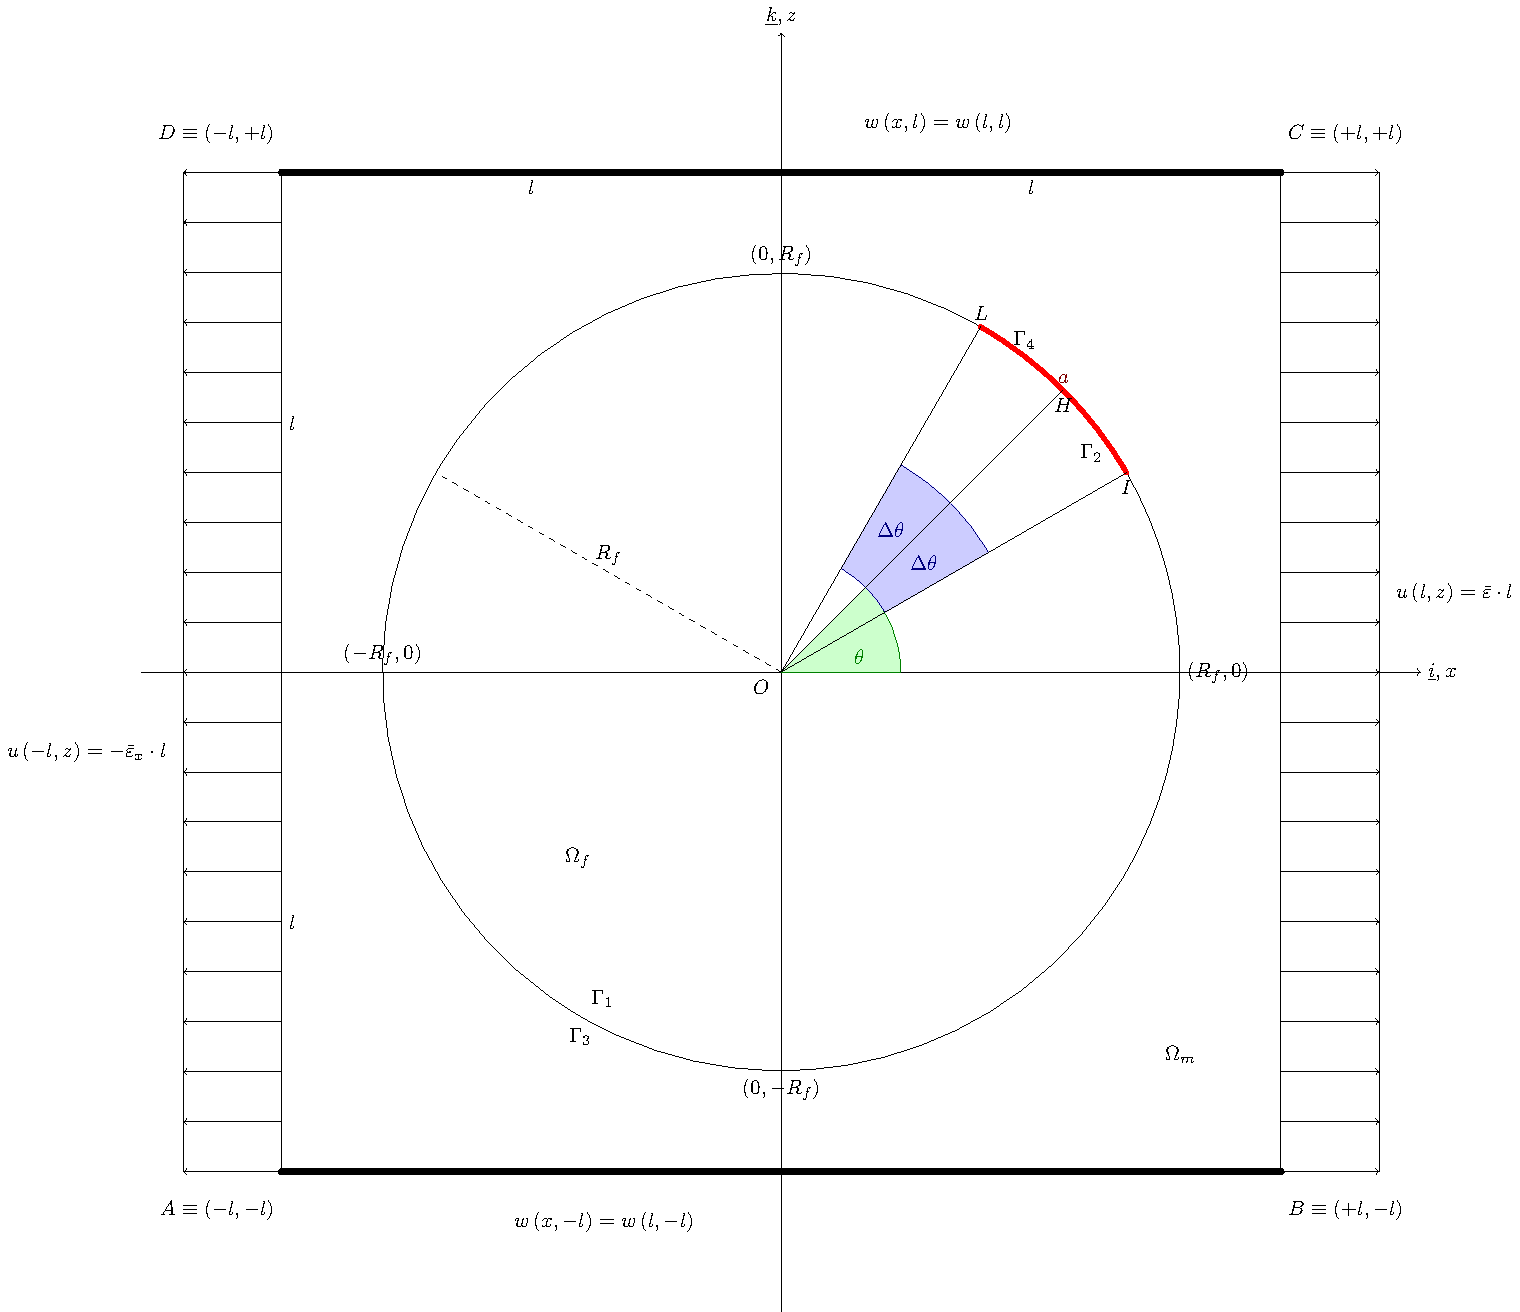
\includegraphics[height=0.7\textheight]{LEFM2DsRVEsFsDdepverdispBCULappAxialDispLR.pdf}
\caption{\scriptsize Isolated RVE with zero vertical displacement BC.}
\label{fig:singleRVE-rigid}
\end{figure}
\end{frame}

\begin{frame}
\frametitle{Reference Models}
\vspace{-0.25cm}
\centering
\begin{figure}
\centering
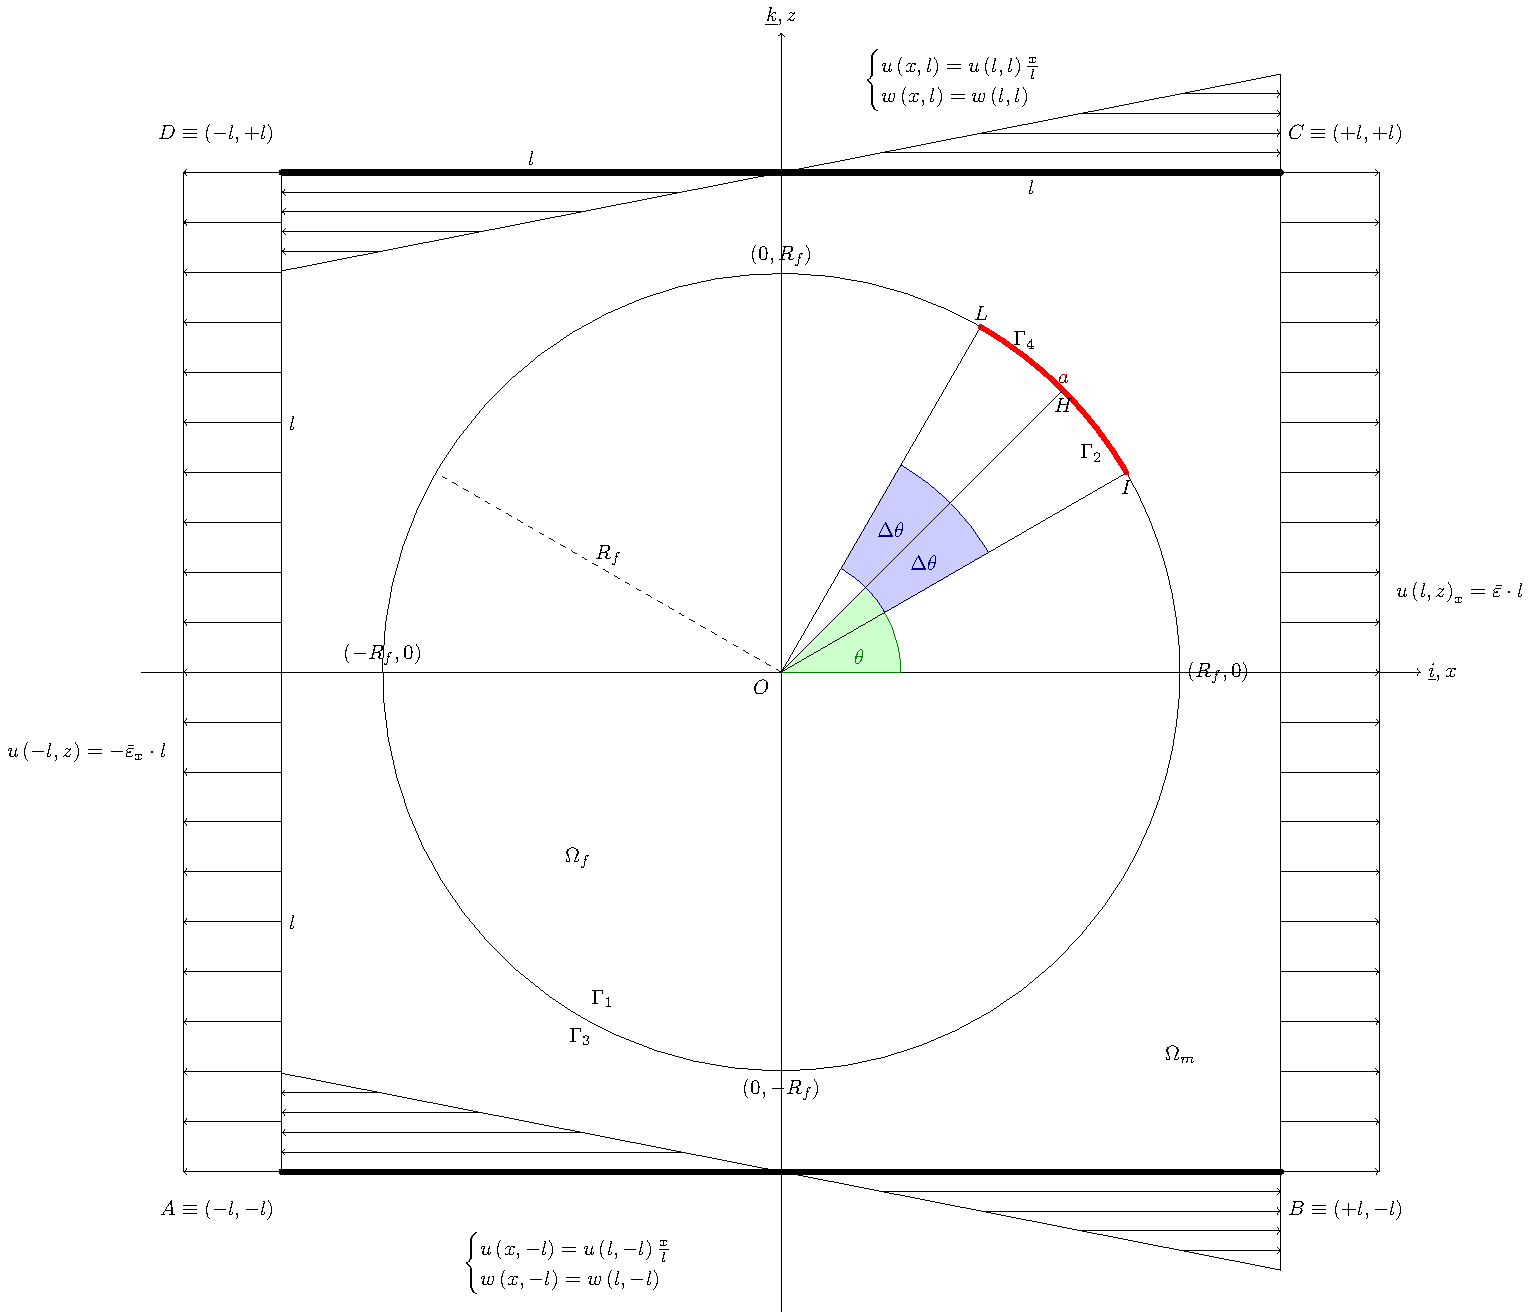
\includegraphics[height=0.7\textheight]{LEFM2DsRVEsFsDhomoBCULappAxialDispLR.pdf}
\caption{\scriptsize Isolated RVE with homogeneous displacement BC.}
\label{fig:singleRVE-homo}
\end{figure}
\end{frame}

\subsection{Angular discretization}

\begin{frame}
\frametitle{Angular discretization}
\vspace{-0.7cm}
\centering
\captionsetup[figure]{font=scriptsize,labelfont=scriptsize}
\begin{figure}[!h]
\centering
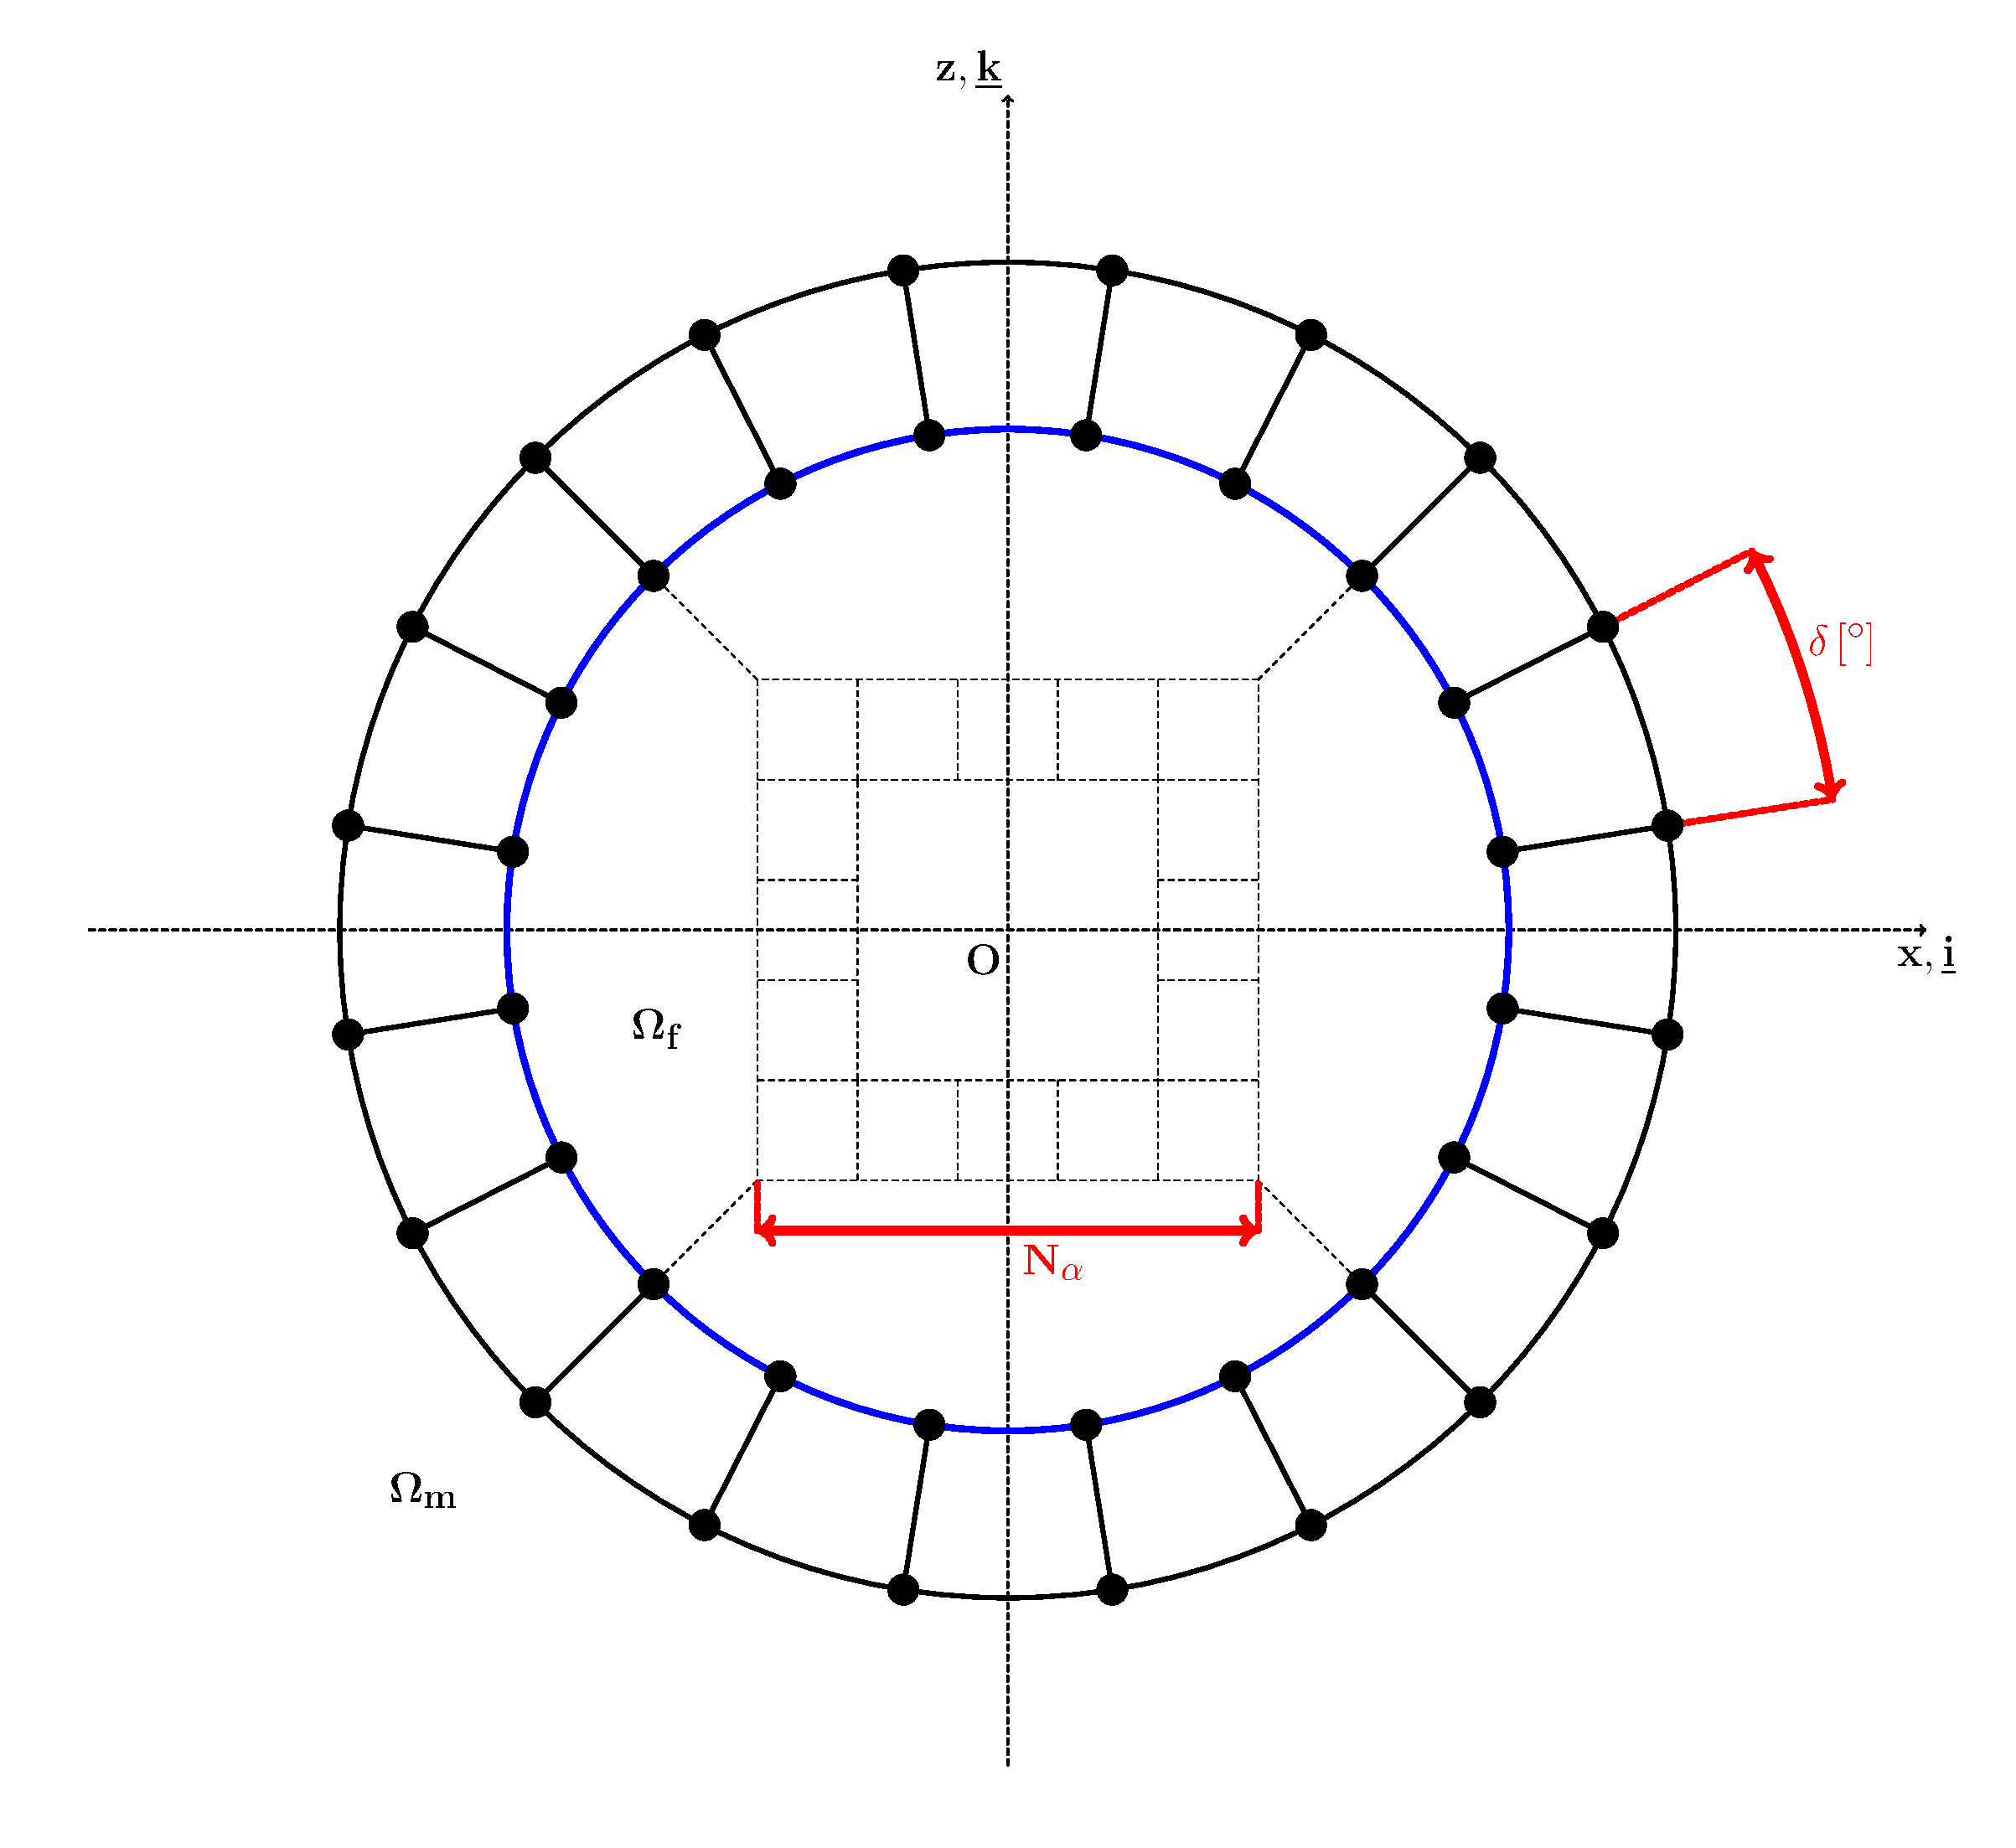
\includegraphics[height=0.7\textheight]{mesh-disc-at-interface.pdf}
  \caption{Angular discretization at fiber/matrix interface: $\delta=\frac{360^{\circ}}{4N_{\alpha}}$.}
  \label{fig:angu-discr-def}
\end{figure}
\end{frame}

\subsection{Materials' properties}

\begin{frame}
\frametitle{Materials' properties}
\vspace{-0.7cm}
\footnotesize
\centering
\captionsetup[figure]{font=scriptsize,labelfont=scriptsize}
\begin{table}[htbp]

  \centering
  %\caption{Single phase properties summary.}
    \begin{tabular}{cccc}

    \textbf{Material} & \textbf{$E\left[GPa\right]$}\ & \textbf{$G\left[GPa\right]$} & \textbf{$\nu\left[-\right]$} \\[3pt]
    \midrule\\[12pt]
    Glass Fiber    & 70,0  & 29,2   & 0,2  \\[16pt]
    Epoxy    & 3,5    & 1,25   & 0,4  

    \end{tabular}%
  \label{tab:phaseprop}%
\end{table}%
\end{frame}

\section{Review of work's progress}

\subsection{Where we were}

\begin{frame}
\frametitle{Where we were}
\vspace{-0.25cm}
\scriptsize
\begin{itemize}[label=\ding{212}]
\item Run simulations with following characteristics:
\begin{table}
\begin{tabular}[!h]{ccc}
\toprule
\midrule
&RUN 1& RUN 2\\
\midrule
BC & $v\left(x,\pm l\right)=0$ & $v\left(x,\pm l\right)=0,\quad u\left(x,\pm l\right)=\frac{u\left(l,\pm l\right)}{l}x$\\[3pt]
$VF_{f}\left[-\right]$&$0.001$&$0.001$\\[3pt]
$\delta$&$1^{\circ}$&$1^{\circ}$\\[3pt]
$\theta$&$0^{\circ}$&$0^{\circ}$\\[3pt]
$\Delta\theta$&$\left[10^{\circ},80^{\circ}\right]$ by $10^{\circ} steps$ &$\left[10^{\circ},80^{\circ}\right]$ by $10^{\circ} steps$ \\[3pt]
Loading&Applied displacement&Applied displacement\\[3pt]
Load&$u\left(\pm l,z\right)=\pm\varepsilon_{xx} l$&$u\left(\pm l,z\right)=\pm\varepsilon_{xx} l$\\[3pt]
&$\varepsilon_{xx}=0.01$&$\varepsilon_{xx}=0.01$\\[3pt]
Material system&Glass fiber/epoxy&Glass fiber/epoxy\\[3pt]
ENRRT calculation&VCCT&VCCT\\
\bottomrule
\end{tabular}
\end{table}
\end{itemize}
\end{frame}

\begin{frame}
\frametitle{Where we were}
\vspace{-0.5cm}
\small
\begin{itemize}[label=\ding{212}]
\item Conclusions from simulations:\\[16pt]
\begin{list}{\Large\textcolor{green}{$\mathbf{\checkmark}$}}{}  
\item Correct global elastic response  
\item Symmetric model gives symmetric results
\item For $VF_{f}\to 0$ boundary conditions are not relevant, same result is obtained
\item Correct order of magnitude of normalized energy release rates
\item Physically sound mode ratio: $G_{I}\uparrow\Delta\theta\downarrow$, $G_{II}\uparrow\Delta\theta\uparrow$
\end{list}
\begin{list}{\Huge\textcolor{red}{$\mathbf{\times}$}}{}  
\item No agreement with BEM results  
\item ENRRTs overestimated 
\end{list}
\end{itemize}
\end{frame}

\subsection{What was to be done}

\begin{frame}
\frametitle{What was to be done}
\vspace{-0.5cm}
\begin{list}{$\text{\rlap{\textcolor{white}{\huge$\mathbf{\checkmark}$}}}\square$}{}  
\item Add J-integral calculations to LEFM models 
\item Add correct treatment of $0^{\circ}$ case
\item Add extraction of stresses and displacements at interface (post-processing)
\item Add extraction of stresses and strains at sections inside the domain (post-processing)
\item Run simulations with refined mesh and J-integral evaluation
\item Analyse simulations' results
\end{list}
\end{frame}

\subsection{Where we are}

\begin{frame}
\frametitle{Where we are}
\vspace{-0.5cm}
\begin{list}{$\text{\rlap{\textcolor{green}{\huge$\mathbf{\checkmark}$}}}\square$}{}  
\item Added J-integral calculations to LEFM models 
\item Added correct treatment of $0^{\circ}$ case
\item Added extraction of stresses and displacements at interface (post-processing)
\item Added extraction of stresses and strains along user-defined radial and circumferential sections inside the domain (post-processing)
\item Run simulations with refined mesh and J-integral evaluation
\item Analysed simulations' results
\end{list}
\end{frame}

\begin{frame}
\frametitle{Where we are}
\vspace{-0.5cm}
\tiny
\begin{table}
\begin{tabular}[!h]{cccc}
\toprule
\midrule
&RUN 1& RUN 2&RUN 3\\
\midrule
BC & $v\left(x,\pm l\right)=0$ & $v\left(x,\pm l\right)=0$&$v\left(x,\pm l\right)=0$\\[6pt]
BC &  & $u\left(x,\pm l\right)=\frac{u\left(l,\pm l\right)}{l}x$&$u\left(x,\pm l\right)=\frac{u\left(l,\pm l\right)}{l}x$\\[6pt]
$VF_{f}\left[-\right]$&$0.001$&$0.001$&$0.001$\\[6pt]
$\delta$&$1^{\circ}$&$1^{\circ}$&$0.4^{\circ}$\\[6pt]
$\theta$&$0^{\circ}$&$0^{\circ}$&$0^{\circ}$\\[6pt]
$\Delta\theta$&$\left[10^{\circ},80^{\circ}\right]$ by $10^{\circ} steps$ &$\left[10^{\circ},80^{\circ}\right]$ by $10^{\circ} steps$  &$\left[0^{\circ},140^{\circ}\right]$ by $5^{\circ} steps$ \\[6pt]
Loading&Applied displacement&Applied displacement&Applied displacement\\[6pt]
Load&$u\left(\pm l,z\right)=\pm\varepsilon_{xx} l$&$u\left(\pm l,z\right)=\pm\varepsilon_{xx} l$&$u\left(\pm l,z\right)=\pm\varepsilon_{xx} l$\\[6pt]
&$\varepsilon_{xx}=0.01$&$\varepsilon_{xx}=0.01$&$\varepsilon_{xx}=0.01$\\[6pt]
Material system&Glass fiber/epoxy&Glass fiber/epoxy&Glass fiber/epoxy\\[6pt]
ENRRT calculation&VCCT&VCCT&VCCT \& J-Integral\\
\bottomrule
\end{tabular}
\end{table}
\end{frame}

\section{Discussion of results}

\subsection{Energy Release Rates by VCCT}

\begin{frame}
\frametitle{\vspace{0.35cm}\scriptsize Energy Release Rates by VCCT}
\vspace{-1.cm}
\begin{figure}
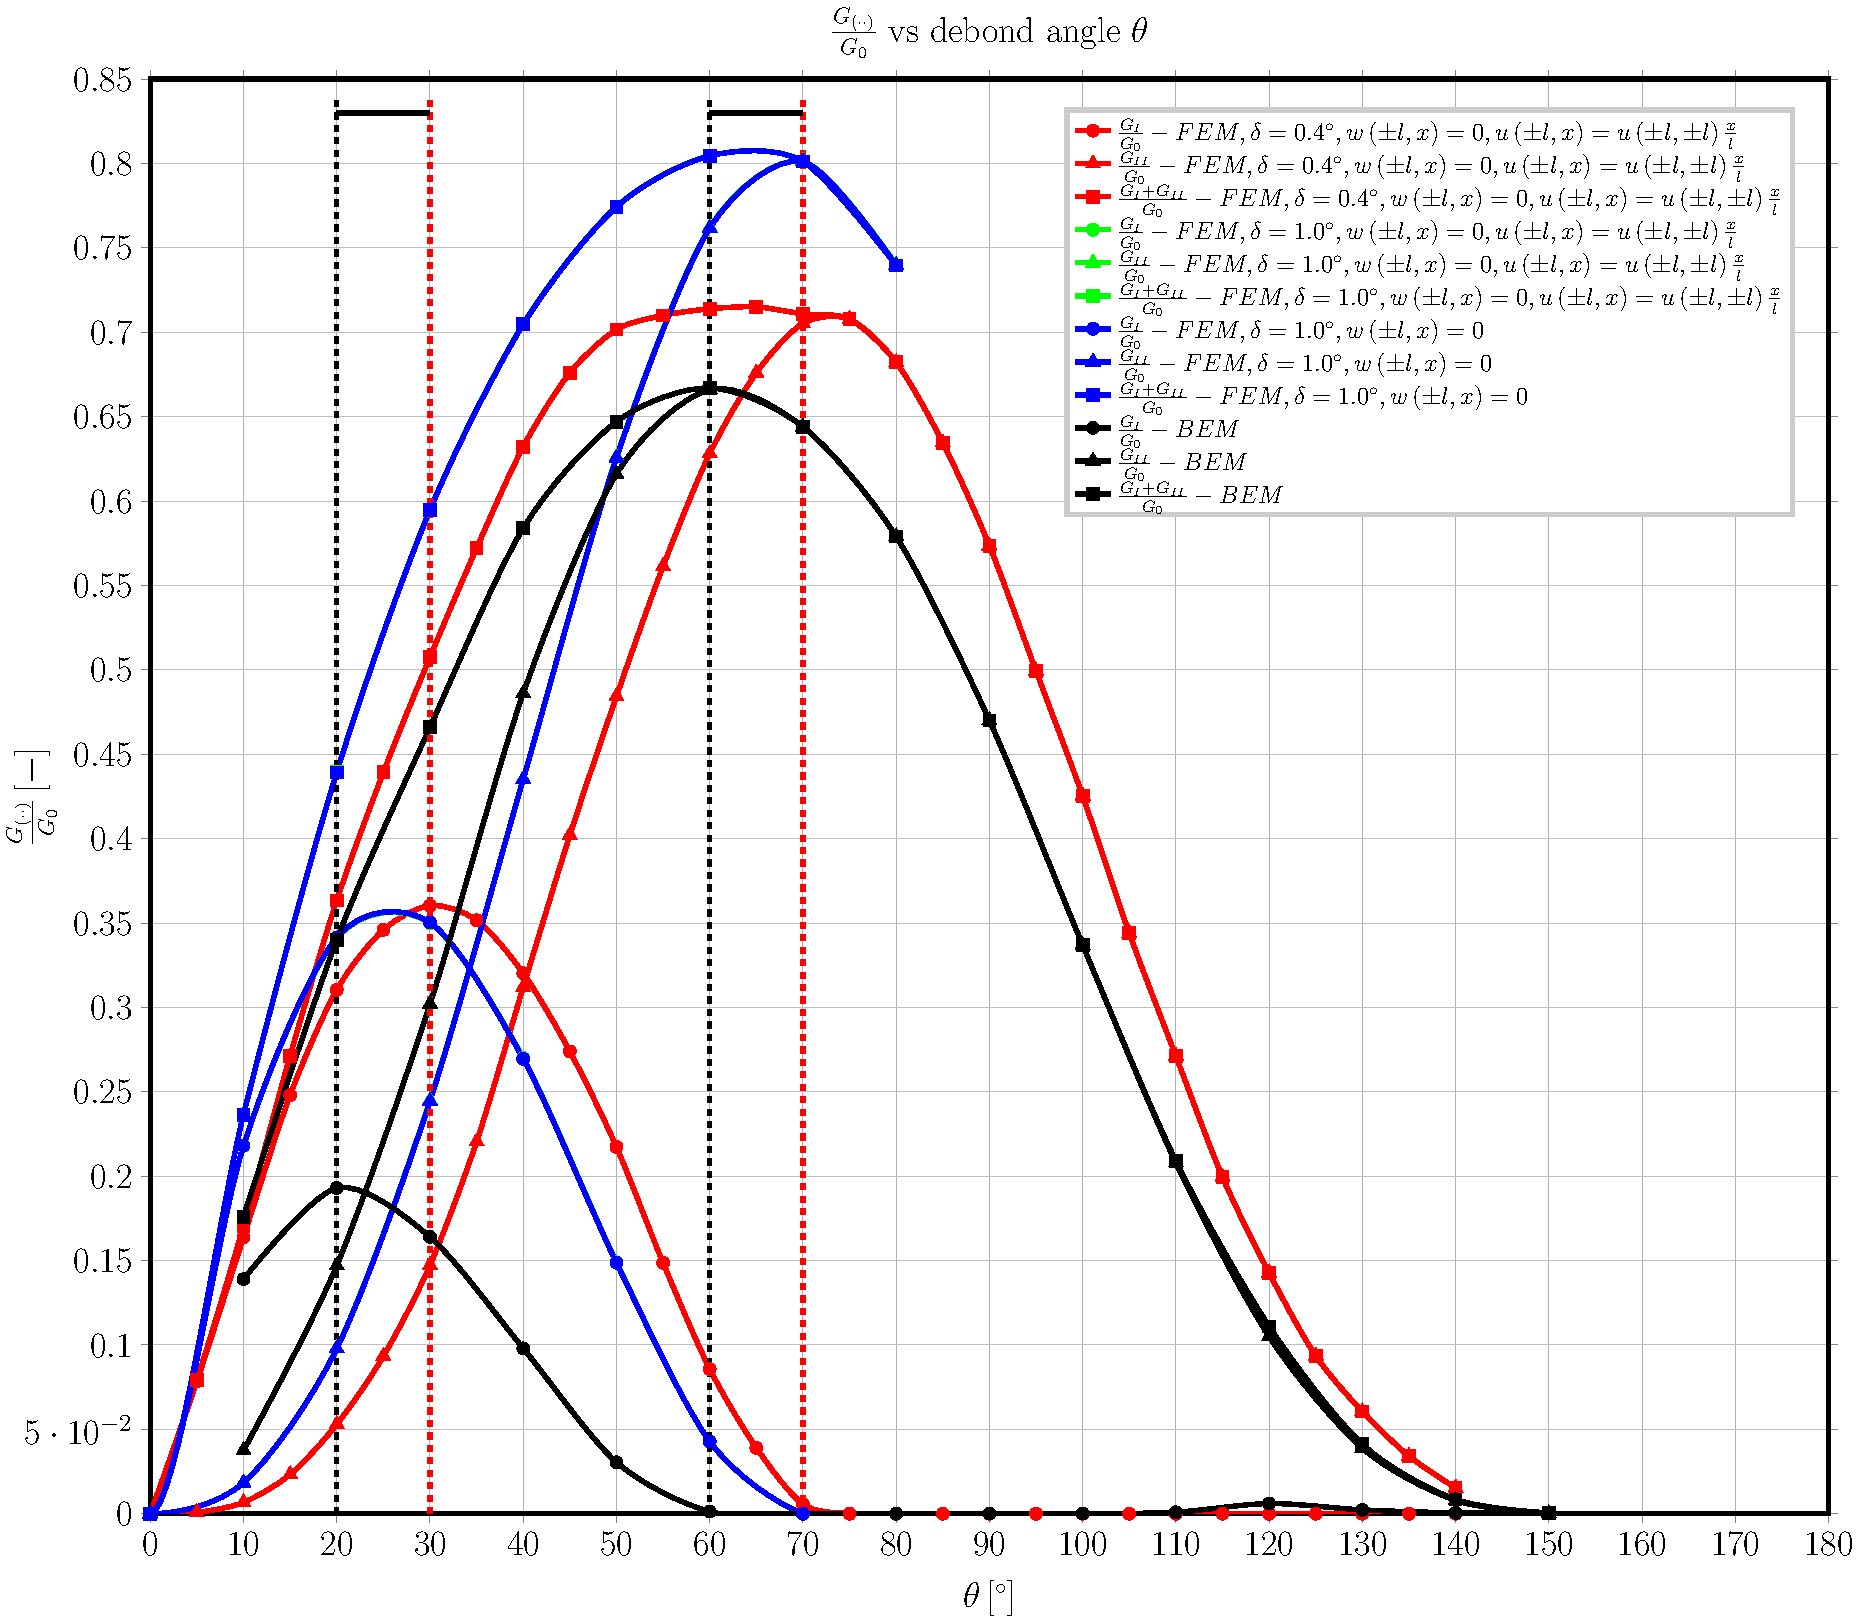
\includegraphics[height=0.9\textheight]{AbqRunSummary_GsoverG0_FEM-BEM-comparison.pdf}
\end{figure}
\end{frame}

\begin{frame}
\frametitle{$G_{c}$ Numerical Evaluation by VCCT}
\vspace{-1.5cm}
\tiny
\centering
\begin{figure}[!h]
\centering
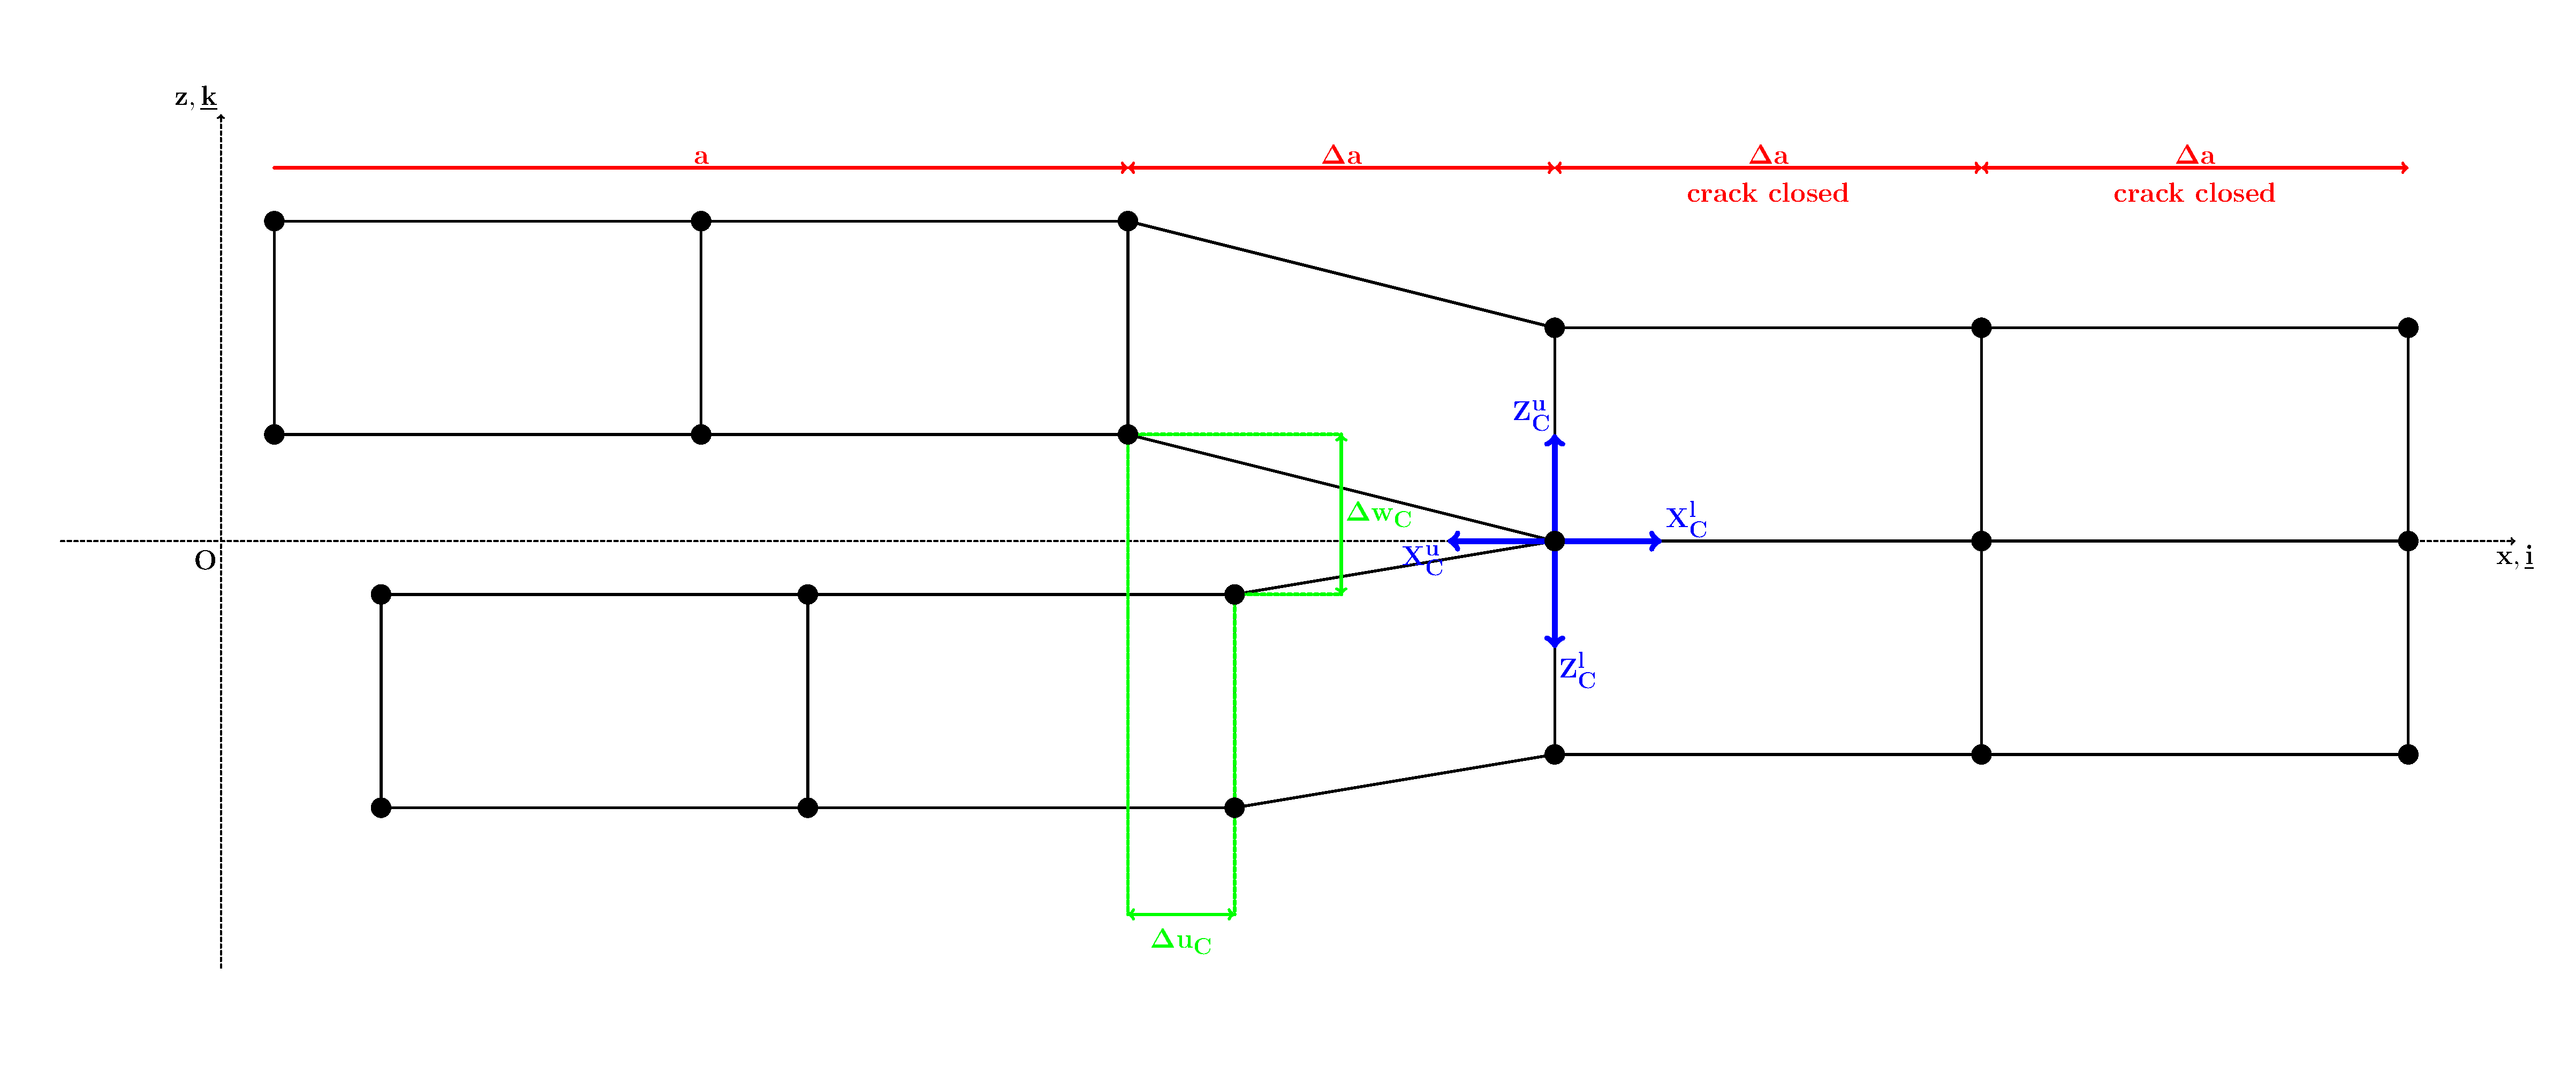
\includegraphics[height=0.6\textheight]{VCCT.pdf}
 % \caption{Angular discretization at fiber/matrix interface.}
  \label{fig:vcct}
\end{figure}
\begin{equation*}
G_{I}=\frac{Z_{C}\Delta w_{C}}{2B\Delta a}=\frac{Z_{C}\left(\Delta w_{C}\right)\Delta w_{C}}{2B\Delta a}\sim G_{I}\left(\Delta w_{C}^{2}\right)\qquad G_{II}=\frac{X_{C}\Delta u_{C}}{2B\Delta a}=\frac{X_{C}\left(\Delta u_{C}\right)\Delta u_{C}}{2B\Delta a}\sim G_{II}\left(\Delta u_{C}^{2}\right)
\end{equation*}
\end{frame}


\begin{frame}
\frametitle{Comments}
\vspace{-0.25cm}
\small
\begin{itemize}[label=\ding{212}]
\item Finer mesh gives results closer to correct ones:
\begin{list}{$\circ$}{} 
\item approximation from above in terms of energy
\item in FEM, the coarser the mesh, the more rigid the system; thus higher energy release
\item for the same number of elements opened at the interface (crack is an ensemble of elements), a larger crack surface is created
\end{list}
\item Values still too big
\item Too much mode I
\item Shift of peaks by $\sim10^{\circ}$
\end{itemize}
\end{frame}

\subsection{Total Energy Release Rate by J-integral}

\begin{frame}
\frametitle{\vspace{0.35cm}\scriptsize Total Energy Release Rate by J-integral}
\vspace{-0.85cm}
\begin{figure}
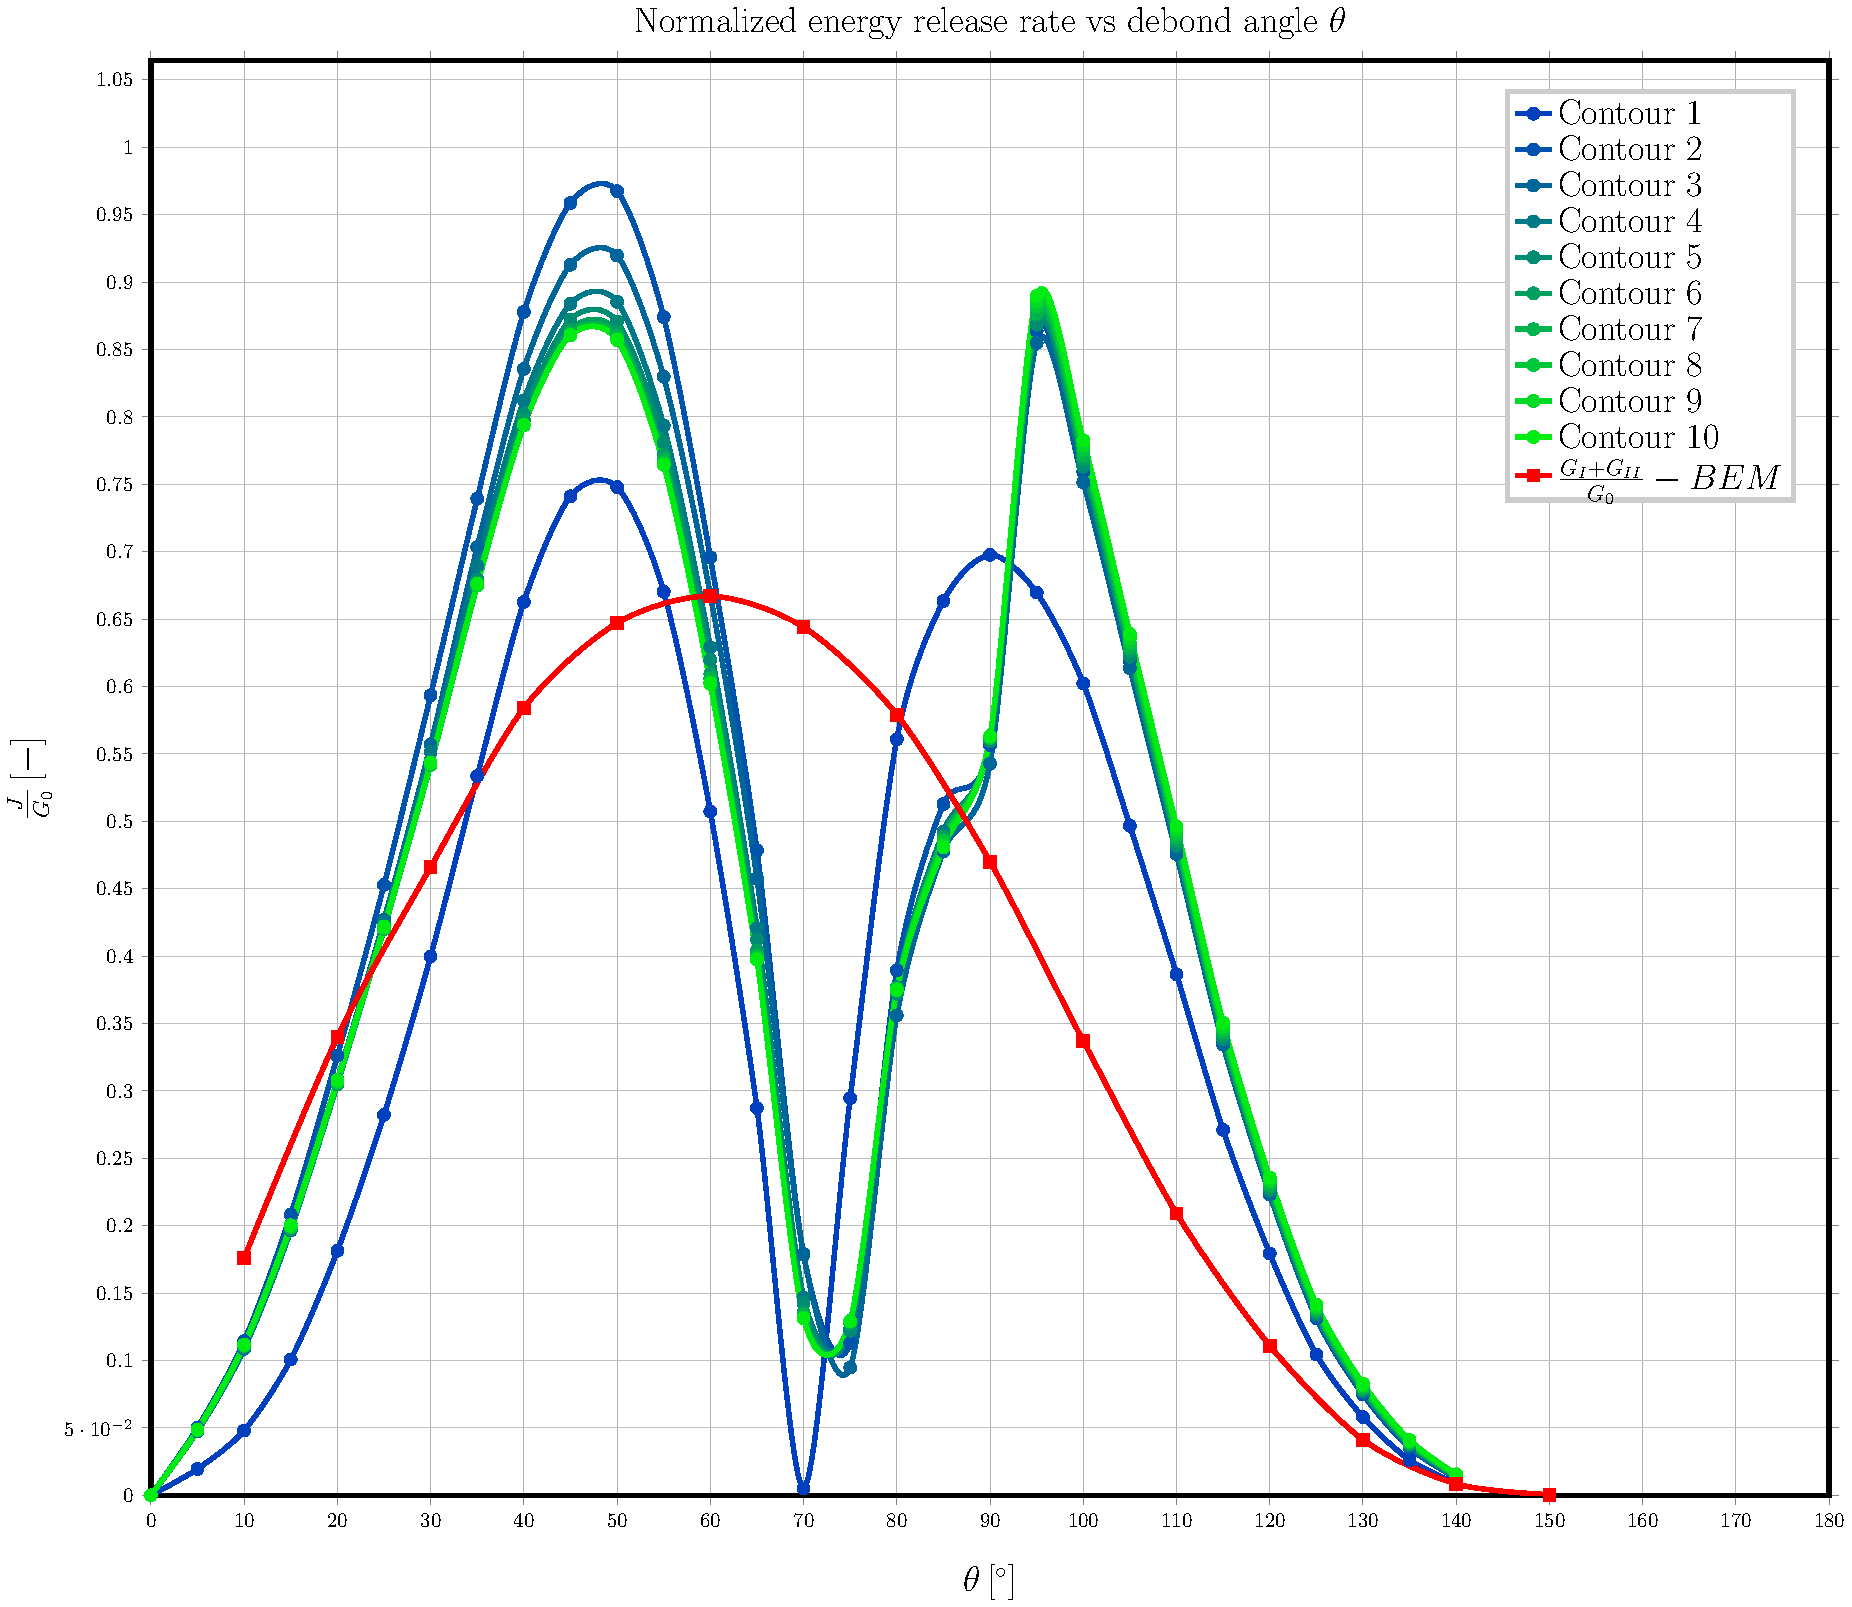
\includegraphics[height=0.9\textheight]{2017-03-03_AbqRunSummary_JsoverG0_FEM-BEM-comparison.pdf}
\end{figure}
\end{frame}

\begin{frame}
\frametitle{Comments}
\vspace{-0.25cm}
\begin{itemize}[label=\ding{212}]
\item Convergence across contour
\item Very far from BEM result
\item Minimum at $\sim 70^{\circ}$, which corresponds to the mode II maximum
\end{itemize}
\end{frame}

\subsection{Interface}

\begin{frame}
\frametitle{\vspace{0.35cm}\scriptsize Interface}
\vspace{-0.85cm}
\begin{figure}
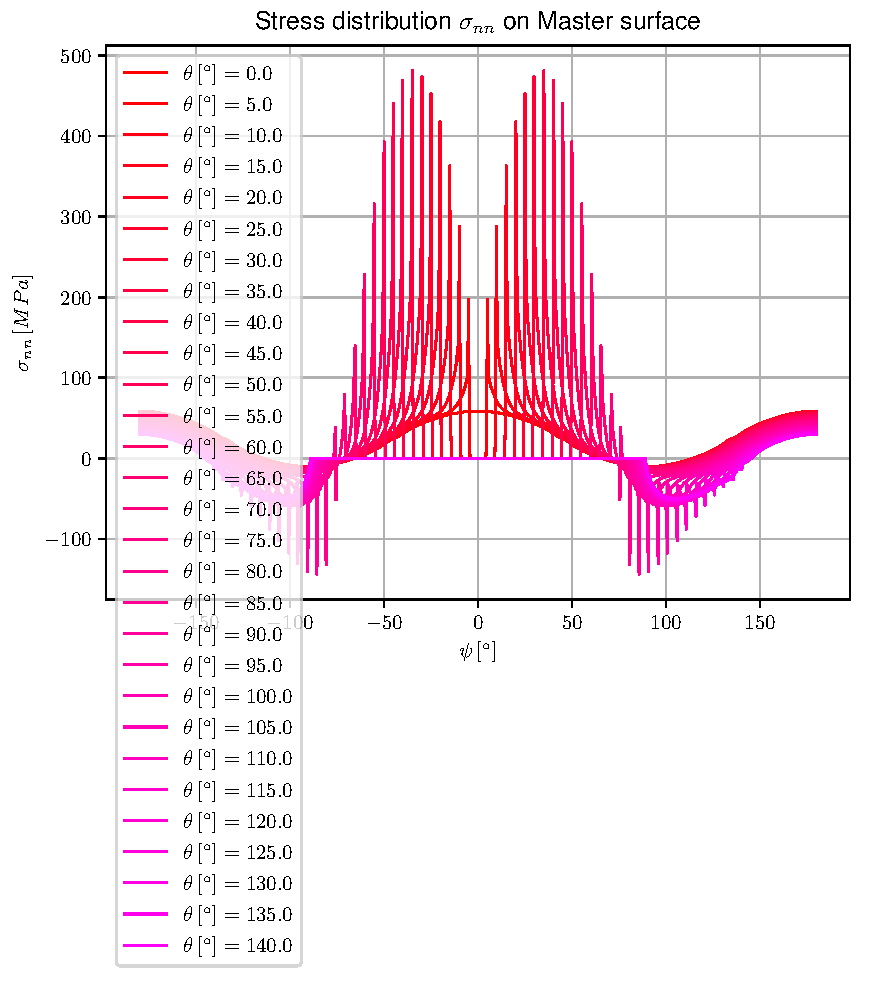
\includegraphics[height=0.9\textheight]{2017-03-03_AbqRunSummary_AllNormalStressOnMaster.pdf}
\end{figure}
\end{frame}

\begin{frame}
\frametitle{\vspace{0.35cm}\scriptsize Interface}
\vspace{-0.85cm}
\begin{figure}
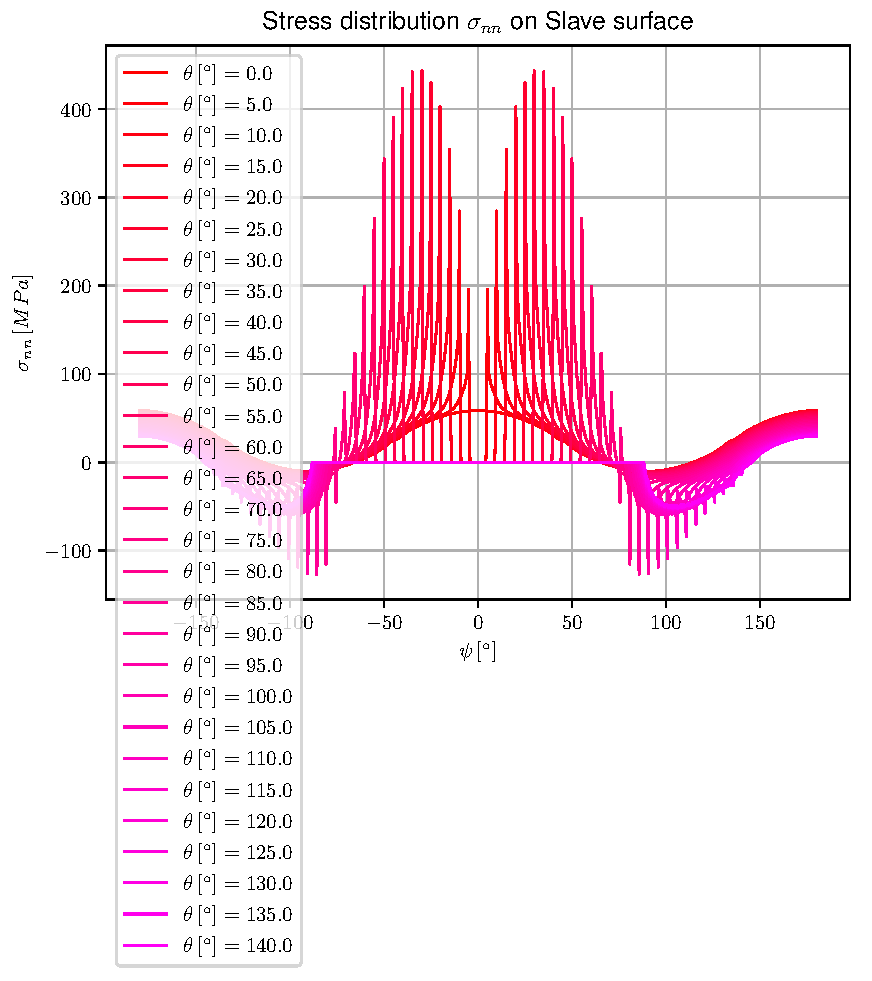
\includegraphics[height=0.9\textheight]{2017-03-03_AbqRunSummary_AllNormalStressOnSlave.pdf}
\end{figure}
\end{frame}

\begin{frame}
\frametitle{\vspace{0.35cm}\scriptsize Interface}
\vspace{-0.85cm}
\begin{figure}
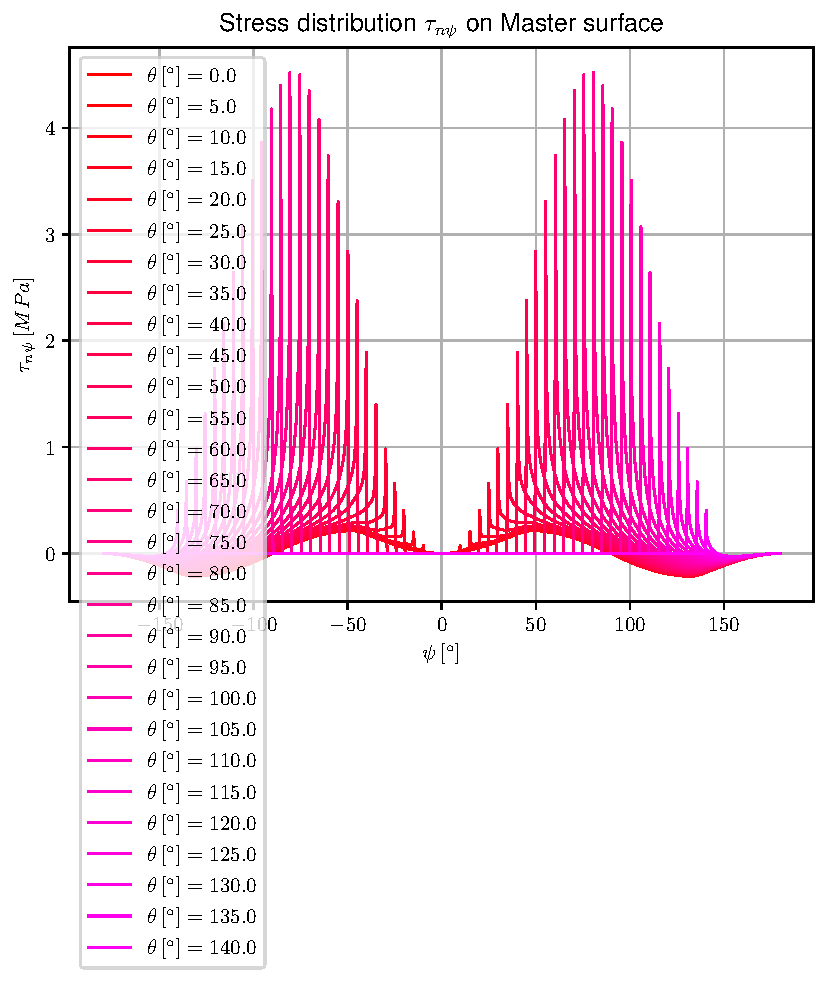
\includegraphics[height=0.9\textheight]{2017-03-03_AbqRunSummary_AllInPlaneShearOnMaster.pdf}
\end{figure}
\end{frame}

\begin{frame}
\frametitle{\vspace{0.35cm}\scriptsize Interface}
\vspace{-0.85cm}
\begin{figure}
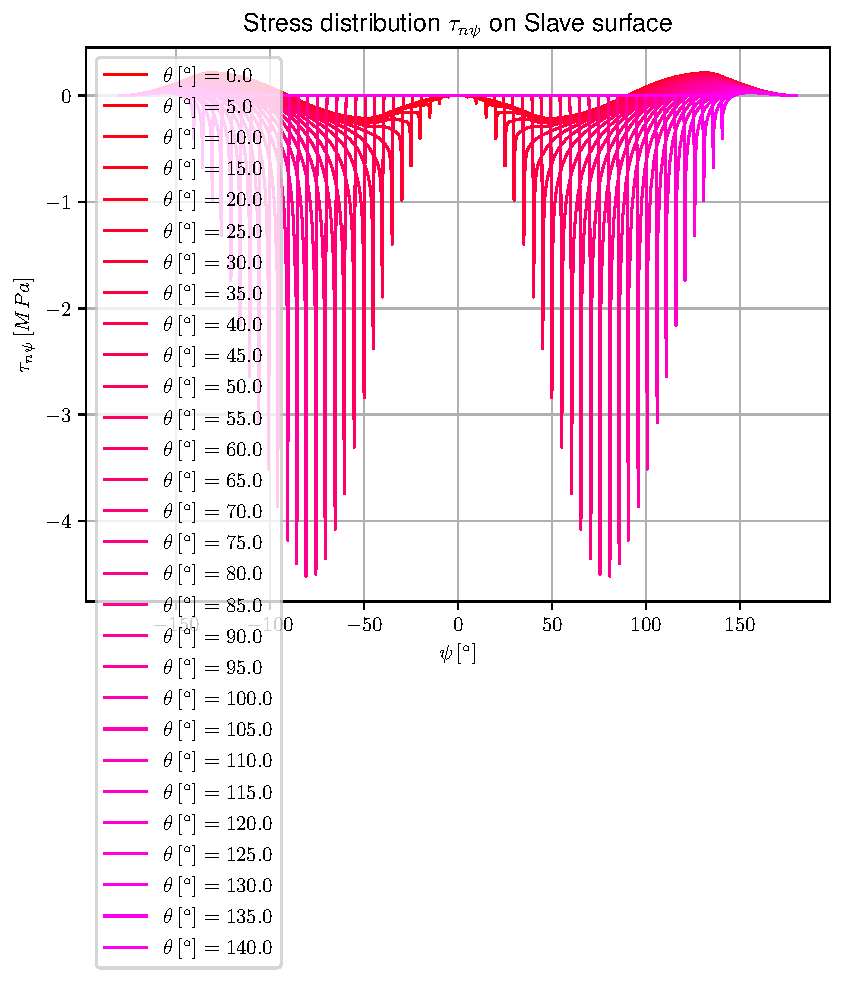
\includegraphics[height=0.9\textheight]{2017-03-03_AbqRunSummary_AllInPlaneShearOnSlave.pdf}
\end{figure}
\end{frame}

\begin{frame}
\frametitle{\vspace{0.35cm}\scriptsize Interface}
\vspace{-0.85cm}
\begin{figure}
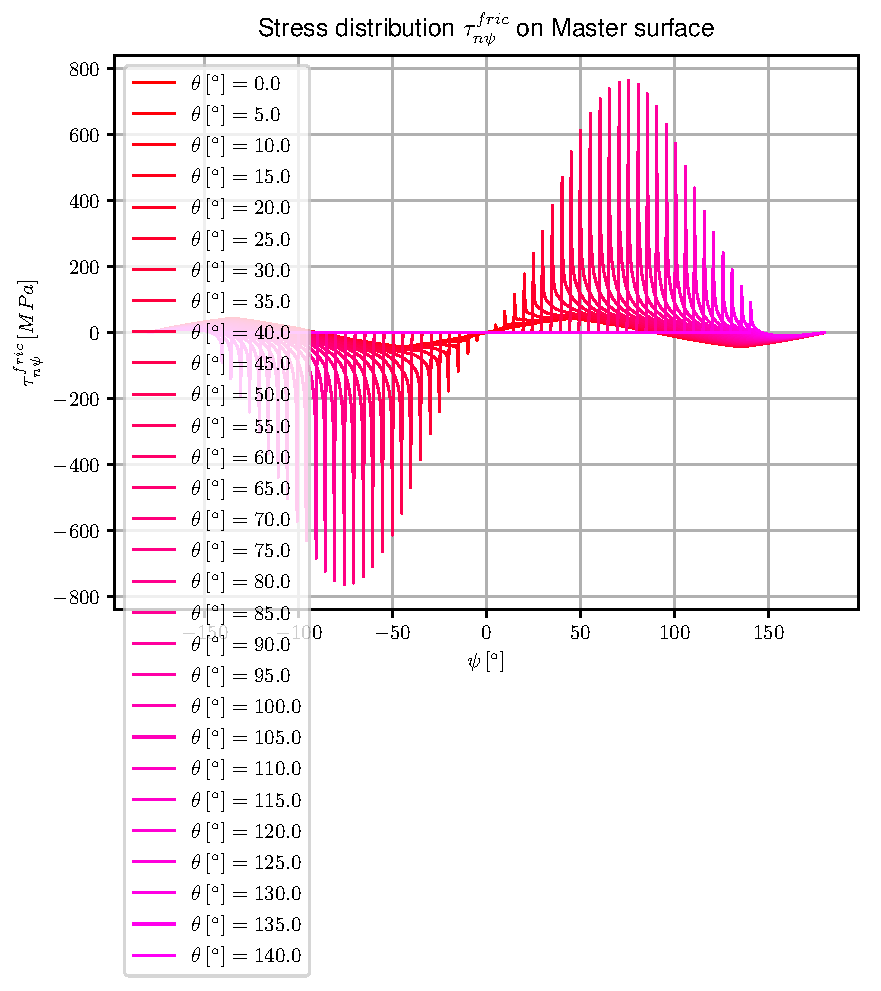
\includegraphics[height=0.9\textheight]{2017-03-03_AbqRunSummary_AllFricShearOnMaster.pdf}
\end{figure}
\end{frame}

\begin{frame}
\frametitle{\vspace{0.35cm}\scriptsize Interface}
\vspace{-0.85cm}
\begin{figure}
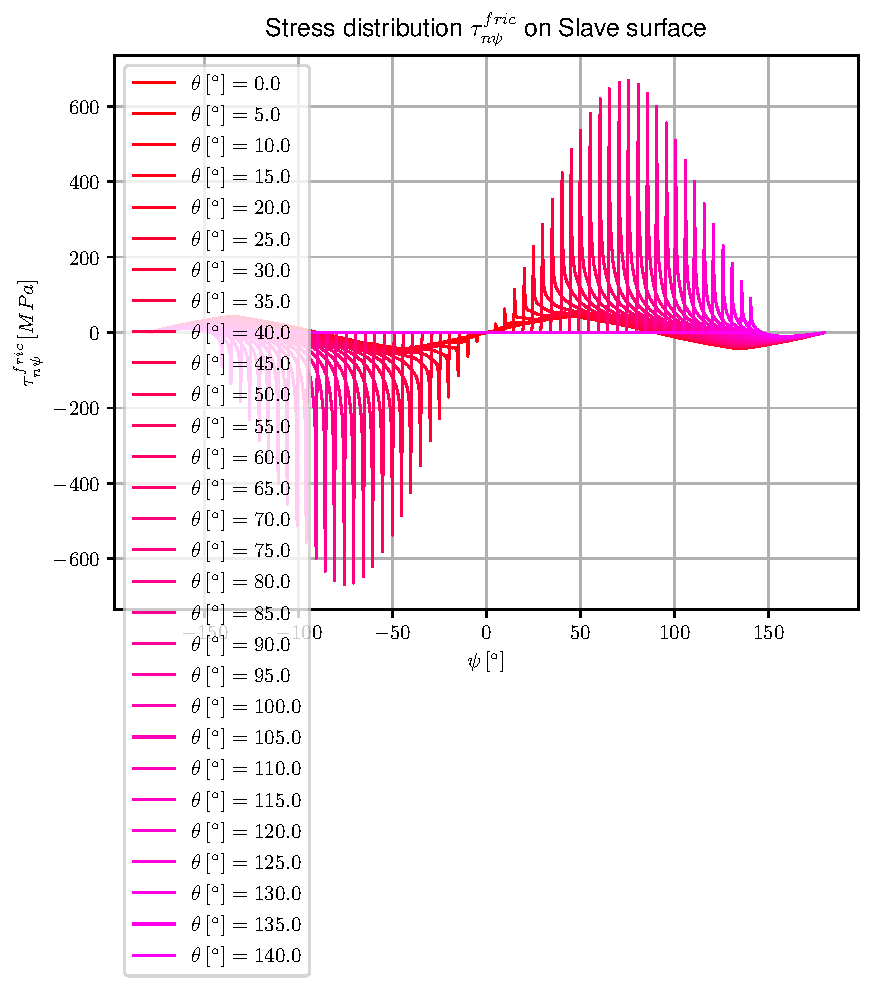
\includegraphics[height=0.9\textheight]{2017-03-03_AbqRunSummary_AllFricShearOnSlave.pdf}
\end{figure}
\end{frame}

\begin{frame}
\frametitle{\vspace{0.35cm}\scriptsize Interface}
\vspace{-0.85cm}
\begin{figure}
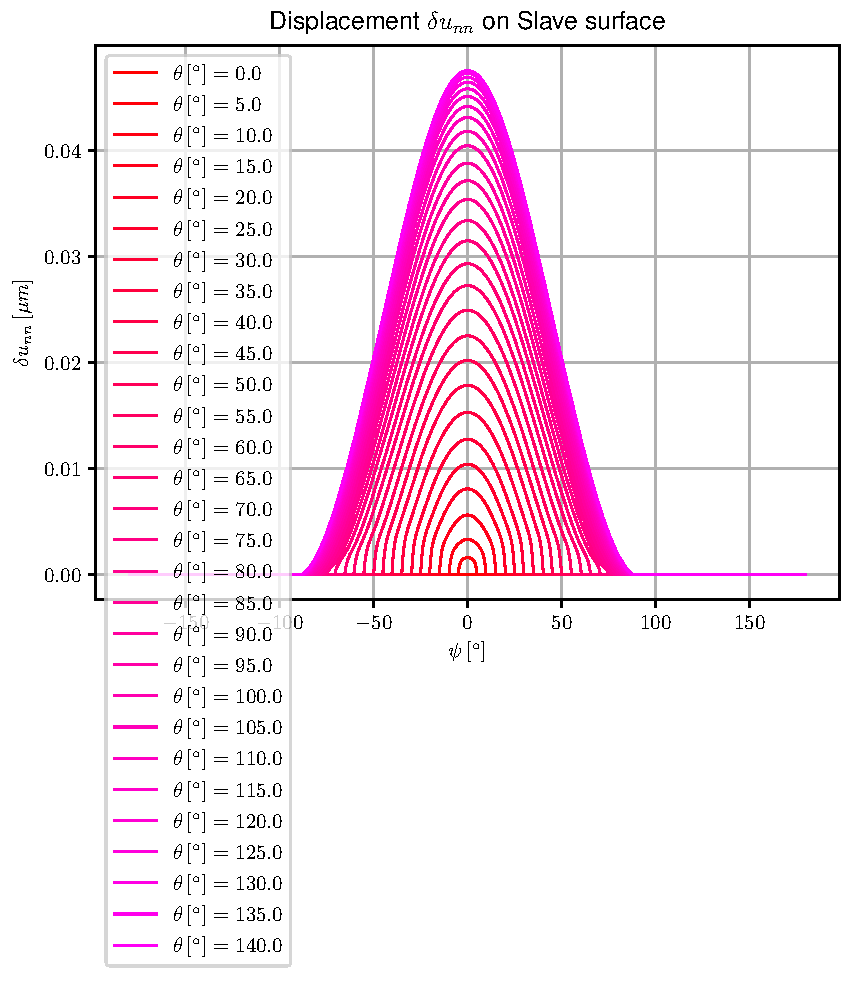
\includegraphics[height=0.9\textheight]{2017-03-03_AbqRunSummary_AllNormalDispsOnSlave.pdf}
\end{figure}
\end{frame}

\begin{frame}
\frametitle{\vspace{0.35cm}\scriptsize Interface}
\vspace{-0.85cm}
\begin{figure}
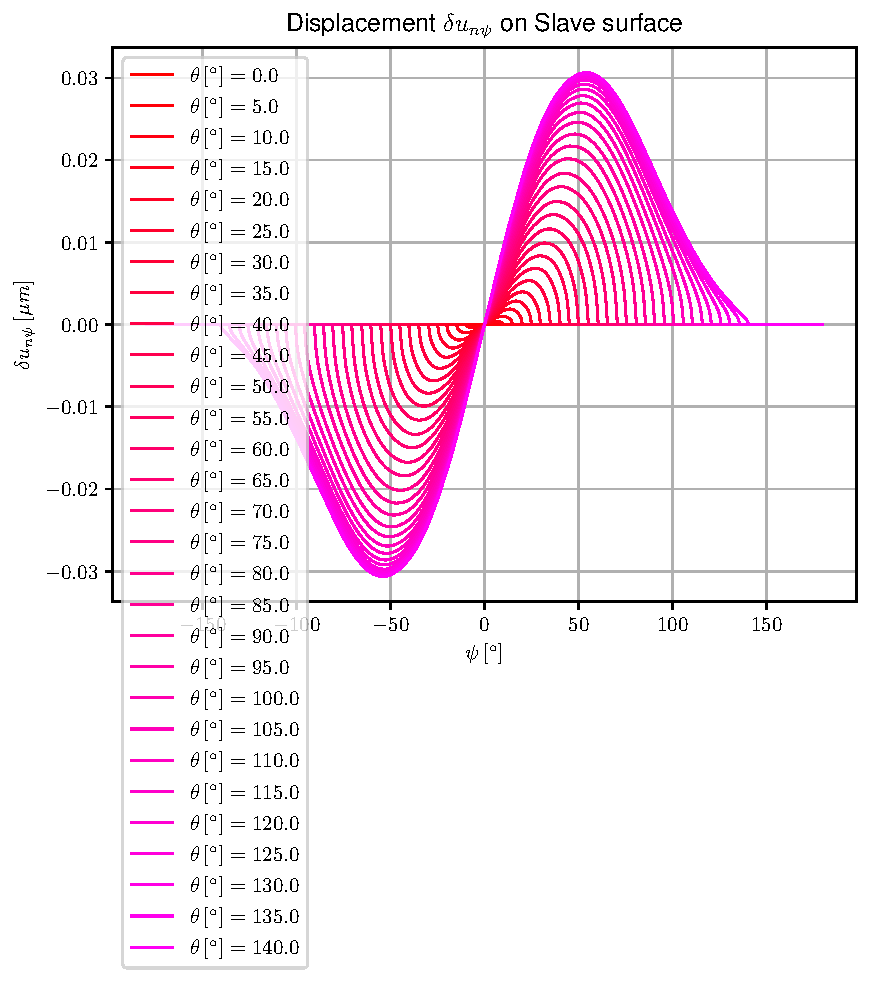
\includegraphics[height=0.9\textheight]{2017-03-03_AbqRunSummary_AllTangentialDispsOnSlave.pdf}
\end{figure}
\end{frame}

\begin{frame}
\frametitle{Comments}
\vspace{-0.25cm}
\begin{itemize}[label=\ding{212}]
\item Periodic distribution with peaks at crack tips
\item Existence of contact zones where crack is open and surfaces slide on each other
\item Shear due to friction
\end{itemize}
\end{frame}

\subsection{Numerical performances}

\begin{frame}
\frametitle{\vspace{0.35cm}\scriptsize Numerical performances}
\vspace{-0.85cm}
\begin{figure}
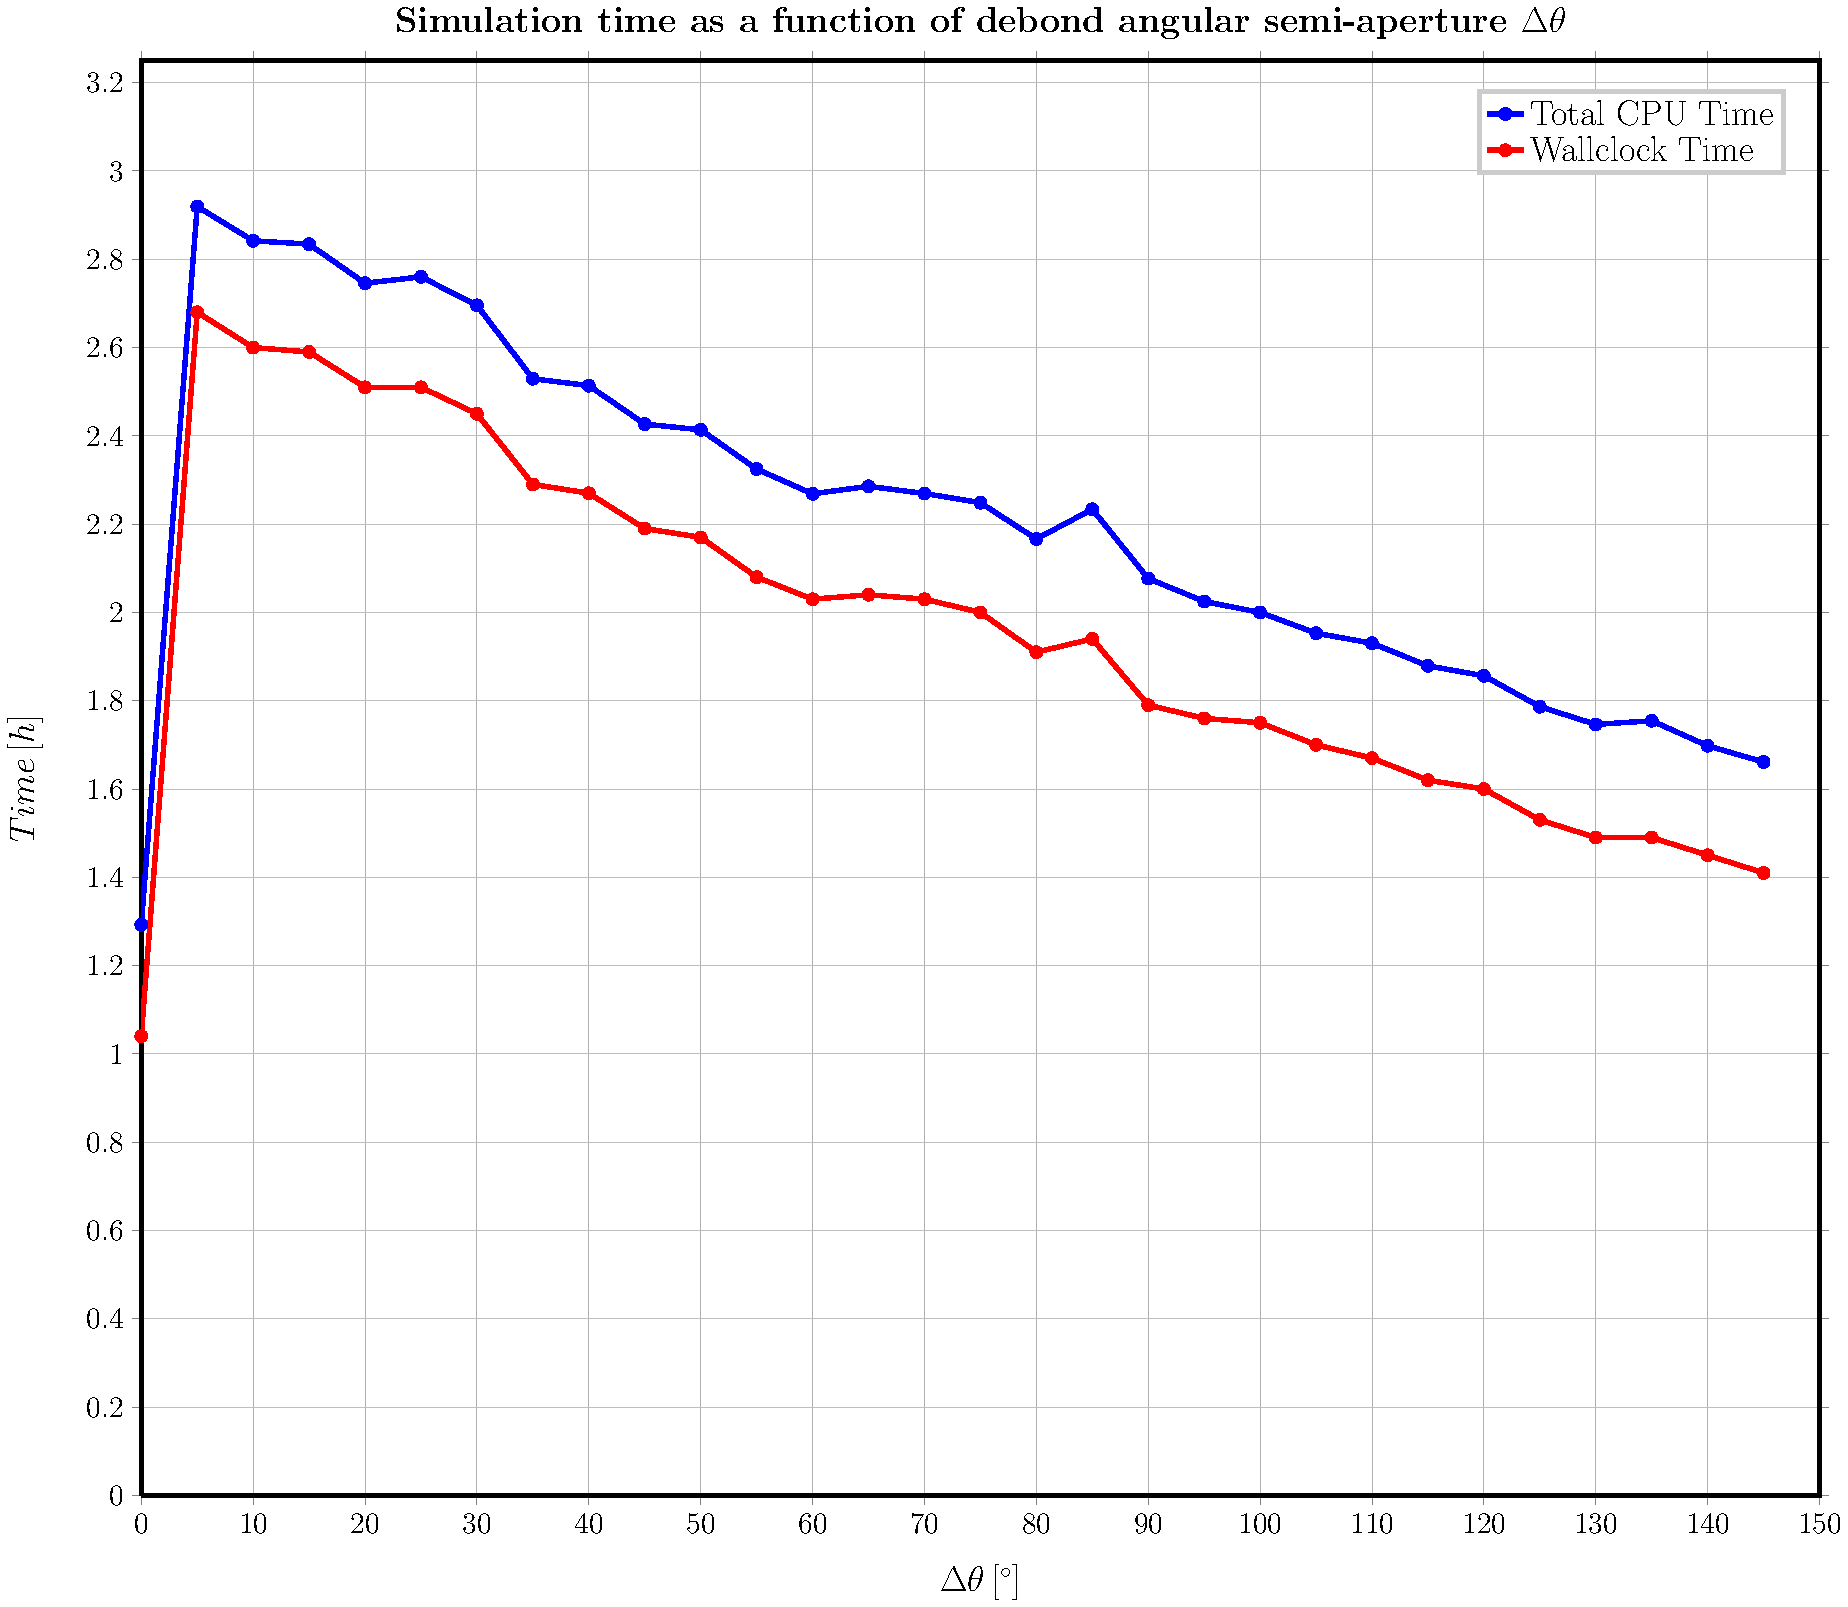
\includegraphics[height=0.9\textheight]{cpus-time.pdf}
\end{figure}
\end{frame}

\begin{frame}
\frametitle{Comments}
\vspace{-0.25cm}
\begin{itemize}[label=\ding{212}]
\item J-integral is highly time-consuming
\item Use of parallelization is only partly effective ($\sim 20\%$ boost) due to contact pair interaction and LEFM evaluations
\end{itemize}
\end{frame}

\subsection{Conclusion}

\begin{frame}
\frametitle{Conclusion}
\vspace{-0.85cm}
\scriptsize
\begin{itemize}[label=\ding{212}]
\item VCCT is optimal wrt J-integral for crack tip determination: Gs are zero everywhere except at crack tips
\item J-integral is not reliable and time-consuming: it should be put aside in favour of VCCT
\item It might be interesting to study J-integral behavior after validation is attained
\item Material properties are the same as Linqi's: they shouldn't be a problem
\item Applied displacement as in Linqi's model: however, value is different $\varepsilon_{xx}=0.01$ (this model) vs $\varepsilon_{xx}=0.05$ (Linqi)
\item Shear due to friction at the interface: just an output? Does it enter the mechanics of the interface?
\item Mesh: do we need a finer mesh? Probably, but it might not be the only variable at play.
\end{itemize}
\end{frame}



%\section{Appendices \& References}
%
%\subsection{Appendices}
%
%
%%\end{frame}
%
%\subsection{References}
%
%\begin{frame}[allowframebreaks]
%  \frametitle{References}
%    
%  \begin{thebibliography}{10}
%    
%%  \beamertemplatebookbibitems
%%  % Start with overview books.
%%
%%  \bibitem{Author1990}
%%    A.~Author.
%%    \newblock {\em Handbook of Everything}.
%%    \newblock Some Press, 1990.
% 
%    
%  \beamertemplatearticlebibitems
%  % Followed by interesting articles. Keep the list short. 
%
%\bibitem{DonaldL.Flaggs1982}
%Donald L. Flaggs, Murat H. Kural;
%\newblock {\em Experimental Determination of the In Situ Transverse Lamina Strength in Graphite/Epoxy Laminates.}
%\newblock Journal of Composite Materials, vol. 16, n. 2, 1982.
%
%\bibitem{Parvizi1978}
%Parvizi A., Bailey J.E;
%\newblock {\em On multiple transverse cracking in glass fibre epoxy cross-ply laminates.}
%\newblock Journal of Materials Science, 1978; 13:2131-2136.
%
%\bibitem{herraez2015}
%Miguel Herr\'aez, Diego Mora, Fernando Naya, Claudio S. Lopes, Carlos Gonz\'alez, Javier LLorca;
%\newblock {\em Transverse cracking of cross-ply laminates: A computational micromechanics perspective.}
%\newblock Composites Science and Technology, 2015; 110:196-204.
%
%\bibitem{Canal2012}
%Luis Pablo Canal, Carlos Gonz\'alez, Javier Segurado, Javier LLorca;
%\newblock {\em Intraply fracture of fiber-reinforced composites: Microscopic mechanisms and modeling.}
%\newblock Composites Science and Technology, 2012; 72(11):1223-1232.
%
%\bibitem{StephenW.Tsai2005}
%Stephen W. Tsai;
%\newblock {\em Thin ply composites.}
%\newblock JEC Magazine 18, 2005.
%
%
%\bibitem{ZnedekP.Bazant2002}
%Znedek P. Bazant;
%\newblock {\em Size Effect Theory and its Application to Fracture of Fiber Composites and Sandwich Plates.} 
%\newblock in Continuum Damage Mechanics of Materials and Structures, eds. O. Allix and F. Hild, 2002.
%
%
%\bibitem{RobinAmacherWayneSmithClemensDransfeldJohnBotsis2014}
%Robin Amacher, Wayne Smith, Clemens Dransfeld, John Botsis, Jo\"el Cugnoni;
%\newblock {\em Thin Ply: from Size-Effect Characterization to Real Life Design}
%\newblock CAMX 2014, 2014
%
%\bibitem{RalfCuntze}
%Ralf Cuntze;
%\newblock {\em The  World-Wide-Failure-Exercises -I  and - II for UD-materials.}
%
%
%\bibitem{Pinho}
%Pinho, S. T. and Pimenta, S.;
%\newblock {\em Size Effects on the Strength and Toughness of Fibre-Reinforced Composites.}
%
%\bibitem{PedroP.CamanhoCarlosG.DavilaSilvestreT.PinhoLorenzoIannucci2006}
%Pedro P. Camanho, Carlos G. D\'avila, Silvestre T. Pinho, Lorenzo Iannucci, Paul Robinson;
%\newblock {\em Prediction of in situ strengths and matrix cracking in composites under transverse tension and in-plane shear.}
%\newblock Composites Part A: Applied Science and Manufacturing, vol. 37, n. 2, 2006.
%
%\bibitem{P.P.CamanhoP.Maimi2007}
%P.P. Camanho, P. Maim\'i, C.G. D\'avila;
%\newblock {\em Prediction of size effects in notched laminates using continuum damage mechanics.}
%\newblock Composites Science and Technology, vol. 67, n. 13, 2007.
%
%\bibitem{Nairn1992}
%J. A. Nairn;
%\newblock {\em The Initiation and Growth of Delaminations Induced by Matrix Microcracks in Laminated Composites.}
%\newblock International Journal of Fracture, vol. 57, 1992.
%
%\bibitem{JoelCugnoniRobinAmacher2013}
%Joel Cugnoni , Robin Amacher, John Botsis;
%\newblock {\em Thin ply technology advantages. An overview of the TPT-TECA project.}
%\newblock 2014.
%
%
%  \end{thebibliography}
%\end{frame}

\begin{frame}[plain]
\frametitle{}
\end{frame}

\end{document}

